
%% Unfortunately for the contents to contain
%% the "Parts" lines successfully, hyperref
%% needs to be disabled.
\documentclass[nohyper, nobib]{tufte-book}
\usepackage{nameref}
% \hypersetup{colorlinks}% uncomment this line if you prefer colored hyperlinks (e.g., for onscreen viewing)

% \usepackage{hyphenat}
\usepackage{url}
\usepackage[backend=biber, natbib=true, style=numeric]{biblatex}
\usepackage{xargs}
\renewcommandx{\cite}[3][1={0pt},2={}]{\sidenote[][#1]{\fullcite[#2]{#3}}}
\usepackage{listings}

\definecolor{codegreen}{rgb}{0,0.6,0}
\definecolor{codegray}{rgb}{0.5,0.5,0.5}
\definecolor{almond}{rgb}{0.94, 0.87, 0.8}
\definecolor{antiquewhite}{rgb}{0.98, 0.92, 0.84}
\lstdefinestyle{mystyle}{ 
    commentstyle=\color{codegreen},
    keywordstyle=\color{magenta},
    backgroundcolor=\color{antiquewhite},
    basicstyle=\ttfamily\footnotesize,
    breakatwhitespace=false,         
    breaklines=true,                 
    captionpos=b,                    
    keepspaces=true,                 
    numbers=left,                    
    numbersep=5pt,                  
    showspaces=false,                
    showstringspaces=false,
}

\lstset{style=mystyle}


\definecolor{eclipseStrings}{RGB}{42,0.0,255}
\definecolor{eclipseKeywords}{RGB}{127,0,85}
\colorlet{numb}{magenta!60!black}

\lstdefinelanguage{json}{
    basicstyle=\normalfont\ttfamily,
    commentstyle=\color{eclipseStrings}, % style of comment
    stringstyle=\color{eclipseKeywords}, % style of strings
    numbers=left,
    numberstyle=\scriptsize,
    stepnumber=1,
    numbersep=8pt,
    showstringspaces=false,
    breaklines=true,
    frame=lines,
    backgroundcolor=\color{gray}, %only if you like
    string=[s]{"}{"},
    comment=[l]{:\ "},
    morecomment=[l]{:"},
    literate=
        *{0}{{{\color{numb}0}}}{1}
         {1}{{{\color{numb}1}}}{1}
         {2}{{{\color{numb}2}}}{1}
         {3}{{{\color{numb}3}}}{1}
         {4}{{{\color{numb}4}}}{1}
         {5}{{{\color{numb}5}}}{1}
         {6}{{{\color{numb}6}}}{1}
         {7}{{{\color{numb}7}}}{1}
         {8}{{{\color{numb}8}}}{1}
         {9}{{{\color{numb}9}}}{1}
}
%%
% Book metadata
\title{Building Production Recommendation Systems in Python,\\ and JAX!}
% \date{The edition number}
\author{Bryan Bischof, Hector Yee}
\publisher{O'reilly Media Inc.}

% Just some sample text
\usepackage{lipsum}

%%
% For nicely typeset tabular material
\usepackage{booktabs}

%%
% For graphics / images
\usepackage{graphicx}
\setkeys{Gin}{width=\linewidth,totalheight=\textheight,keepaspectratio}
\graphicspath{{graphics/}}

% The fancyvrb package lets us customize the formatting of verbatim
% environments.  We use a slightly smaller font.
\usepackage{fancyvrb}
\fvset{fontsize=\normalsize}

%%
% Prints argument within hanging parentheses (i.e., parentheses that take
% up no horizontal space).  Useful in tabular environments.
\newcommand{\hangp}[1]{\makebox[0pt][r]{(}#1\makebox[0pt][l]{)}}

%%
% Prints an asterisk that takes up no horizontal space.
% Useful in tabular environments.
\newcommand{\hangstar}{\makebox[0pt][l]{*}}

%%
% Prints a trailing space in a smart way.
\usepackage{xspace}

%%
% Some shortcuts for Tufte's book titles.  The lowercase commands will
% produce the initials of the book title in italics.  The all-caps commands
% will print out the full title of the book in italics.
\newcommand{\vdqi}{\textit{VDQI}\xspace}
\newcommand{\ei}{\textit{EI}\xspace}
\newcommand{\ve}{\textit{VE}\xspace}
\newcommand{\be}{\textit{BE}\xspace}
\newcommand{\VDQI}{\textit{The Visual Display of Quantitative Information}\xspace}
\newcommand{\EI}{\textit{Envisioning Information}\xspace}
\newcommand{\VE}{\textit{Visual Explanations}\xspace}
\newcommand{\BE}{\textit{Beautiful Evidence}\xspace}

\newcommand{\TL}{Tufte-\LaTeX\xspace}

% Prints the month name (e.g., January) and the year (e.g., 2008)
\newcommand{\monthyear}{%
  \ifcase\month\or January\or February\or March\or April\or May\or June\or
  July\or August\or September\or October\or November\or
  December\fi\space\number\year
}


% Prints an epigraph and speaker in sans serif, all-caps type.
\newcommand{\openepigraph}[2]{%
  %\sffamily\fontsize{14}{16}\selectfont
  \begin{fullwidth}
  \sffamily\large
  \begin{doublespace}
  \noindent\allcaps{#1}\\% epigraph
  \noindent\allcaps{#2}% author
  \end{doublespace}
  \end{fullwidth}
}

% Inserts a blank page
\newcommand{\blankpage}{\newpage\hbox{}\thispagestyle{empty}\newpage}

\usepackage{units}

% Typesets the font size, leading, and measure in the form of 10/12x26 pc.
\newcommand{\measure}[3]{#1/#2$\times$\unit[#3]{pc}}

% Macros for typesetting the documentation
\newcommand{\hlred}[1]{\textcolor{Maroon}{#1}}% prints in red
\newcommand{\hangleft}[1]{\makebox[0pt][r]{#1}}
\newcommand{\hairsp}{\hspace{1pt}}% hair space
\newcommand{\hquad}{\hskip0.5em\relax}% half quad space
\newcommand{\TODO}{\textcolor{red}{\bf TODO!}\xspace}
\newcommand{\ie}{\textit{i.\hairsp{}e.}\xspace}
\newcommand{\eg}{\textit{e.\hairsp{}g.}\xspace}
\newcommand{\na}{\quad--}% used in tables for N/A cells
\providecommand{\XeLaTeX}{X\lower.5ex\hbox{\kern-0.15em\reflectbox{E}}\kern-0.1em\LaTeX}
\newcommand{\tXeLaTeX}{\XeLaTeX\index{XeLaTeX@\protect\XeLaTeX}}
% \index{\texttt{\textbackslash xyz}@\hangleft{\texttt{\textbackslash}}\texttt{xyz}}
\newcommand{\tuftebs}{\symbol{'134}}% a backslash in tt type in OT1/T1
\newcommand{\doccmdnoindex}[2][]{\texttt{\tuftebs#2}}% command name -- adds backslash automatically (and doesn't add cmd to the index)
\newcommand{\doccmddef}[2][]{%
  \hlred{\texttt{\tuftebs#2}}\label{cmd:#2}%
  \ifthenelse{\isempty{#1}}%
    {% add the command to the index
      \index{#2 command@\protect\hangleft{\texttt{\tuftebs}}\texttt{#2}}% command name
    }%
    {% add the command and package to the index
      \index{#2 command@\protect\hangleft{\texttt{\tuftebs}}\texttt{#2} (\texttt{#1} package)}% command name
      \index{#1 package@\texttt{#1} package}\index{packages!#1@\texttt{#1}}% package name
    }%
}% command name -- adds backslash automatically
\newcommand{\doccmd}[2][]{%
  \texttt{\tuftebs#2}%
  \ifthenelse{\isempty{#1}}%
    {% add the command to the index
      \index{#2 command@\protect\hangleft{\texttt{\tuftebs}}\texttt{#2}}% command name
    }%
    {% add the command and package to the index
      \index{#2 command@\protect\hangleft{\texttt{\tuftebs}}\texttt{#2} (\texttt{#1} package)}% command name
      \index{#1 package@\texttt{#1} package}\index{packages!#1@\texttt{#1}}% package name
    }%
}% command name -- adds backslash automatically
\newcommand{\docopt}[1]{\ensuremath{\langle}\textrm{\textit{#1}}\ensuremath{\rangle}}% optional command argument
\newcommand{\docarg}[1]{\textrm{\textit{#1}}}% (required) command argument
\newenvironment{docspec}{\begin{quotation}\ttfamily\parskip0pt\parindent0pt\ignorespaces}{\end{quotation}}% command specification environment
\newcommand{\docenv}[1]{\texttt{#1}\index{#1 environment@\texttt{#1} environment}\index{environments!#1@\texttt{#1}}}% environment name
\newcommand{\docenvdef}[1]{\hlred{\texttt{#1}}\label{env:#1}\index{#1 environment@\texttt{#1} environment}\index{environments!#1@\texttt{#1}}}% environment name
\newcommand{\docpkg}[1]{\texttt{#1}\index{#1 package@\texttt{#1} package}\index{packages!#1@\texttt{#1}}}% package name
\newcommand{\doccls}[1]{\texttt{#1}}% document class name
\newcommand{\docclsopt}[1]{\texttt{#1}\index{#1 class option@\texttt{#1} class option}\index{class options!#1@\texttt{#1}}}% document class option name
\newcommand{\docclsoptdef}[1]{\hlred{\texttt{#1}}\label{clsopt:#1}\index{#1 class option@\texttt{#1} class option}\index{class options!#1@\texttt{#1}}}% document class option name defined
\newcommand{\docmsg}[2]{\bigskip\begin{fullwidth}\noindent\ttfamily#1\end{fullwidth}\medskip\par\noindent#2}
\newcommand{\docfilehook}[2]{\texttt{#1}\index{file hooks!#2}\index{#1@\texttt{#1}}}
\newcommand{\doccounter}[1]{\texttt{#1}\index{#1 counter@\texttt{#1} counter}}

% Generates the index
\usepackage{makeidx}
\makeindex

%%%% Kevin Godny's code for title page and contents from https://groups.google.com/forum/#!topic/tufte-latex/ujdzrktC1BQ
\makeatletter
\renewcommand{\maketitlepage}{%
\begingroup%
\setlength{\parindent}{0pt}

{\fontsize{24}{24}\selectfont\textit{\@author}\par}

\vspace{1.75in}{\fontsize{36}{54}\selectfont\@title\par}

\vspace{0.5in}{\fontsize{14}{14}\selectfont\textsf{\smallcaps{\@date}}\par}

\vfill{\fontsize{14}{14}\selectfont\textit{\@publisher}\par}

\thispagestyle{empty}
\endgroup
}
\makeatother

\titlecontents{part}%
    [0pt]% distance from left margin
    {\addvspace{0.25\baselineskip}}% above (global formatting of entry)
    {\allcaps{Part~\thecontentslabel}\allcaps}% before w/ label (label = ``Part I'')
    {\allcaps{Part~\thecontentslabel}\allcaps}% before w/o label
    {}% filler and page (leaders and page num)
    [\vspace*{0.5\baselineskip}]% after

\titlecontents{chapter}%
    [4em]% distance from left margin
    {}% above (global formatting of entry)
    {\contentslabel{2em}\textit}% before w/ label (label = ``Chapter 1'')
    {\hspace{0em}\textit}% before w/o label
    {\qquad\thecontentspage}% filler and page (leaders and page num)
    [\vspace*{0.5\baselineskip}]% after
    
%%%% End additional code by Kevin Godby

\begin{document}

% Front matter
\frontmatter

% r.3 full title page
\maketitle

% v.4 copyright page
\newpage
\begin{fullwidth}
~\vfill
\thispagestyle{empty}
\setlength{\parindent}{0pt}
\setlength{\parskip}{\baselineskip}
Copyright \copyright\ \the\year\ \thanklessauthor

\par\smallcaps{Published by \thanklesspublisher}

% \par\smallcaps{tufte-latex.googlecode.com}

% \par Licensed under the Apache License, Version 2.0 (the ``License''); you may not
% use this file except in compliance with the License. You may obtain a copy
% of the License at \url{http://www.apache.org/licenses/LICENSE-2.0}. Unless
% required by applicable law or agreed to in writing, software distributed
% under the License is distributed on an \smallcaps{``AS IS'' BASIS, WITHOUT
% WARRANTIES OR CONDITIONS OF ANY KIND}, either express or implied. See the
% License for the specific language governing permissions and limitations
% under the License.\index{license}

% \par\textit{First printing, \monthyear}
\end{fullwidth}

% r.5 contents
\tableofcontents

% \listoffigures

% \listoftables


\chapter*{Preface}

How did you come to find this book? Did you see an ad for it on some website? Maybe a friend or instructor suggested it; or perhaps you saw a tweet referencing it. Could it be that you found it sitting on a shelf in a bookstore; a bookstore that your trusty maps app led you to. In any case, you’ve almost certainly come to this book via a recommendation system.

Implementing and designing systems to provide suggestions to users is among the most popular and most essential first applications of Machine Learning to any business. Whether you wish to help your users find the best clothing to their tastes, the most appealing items to buy from your online store, the videos to enrich and entertain them, maximally engaging content from their networks, or the news they need to know on that day, recommendation systems(often abbreviated RecSys) provide the way.

Modern recommendation system designs are as diverse as the fields in which they serve. Methods for recommending can come from traditional statistical learning algorithms, linear algebraic inspirations, geometric considerations, and, of course, gradient based methods. While the algorithmic methods are diverse, so too are the statistical and evaluation considerations for recommending: personalized ranking, search recommendations, sequence modeling, and the scoring for all of the above are now need-to-know for the working ML Engineer in the space of recommendation systems.

As a practitioner, you’ll need to understand:
\begin{itemize}
    \item What are the essential data to get started building a RecSys
    \item How to take your data and business problem, and frame it as a RecSys problem
    \item What are the appropriate models for your RecSys problem and how should you evaluate them
    \item How to implement, train, test, and deploy the aforementioned model
    \item What metrics you should be tracking to ensure your system is working as planned
    \item How to incrementally improve your system as you learn more about your users, products, and business case
\end{itemize}

This book seeks to illustrate the core concepts and examples necessary to do the above–whatever the industry or scale. In this book we guide the reader through the math, ideas, and implementation details of your first or fiftieth recommendation system. We illustrate how to build these systems with Python and JAX.

% r.9 introduction
\cleardoublepage

%%
% Start the main matter (normal chapters)
\mainmatter

\part{The Warmup}

\chapter{Definition and Introduction}
\label{ch:introduction}

\section{What on earth are we doing here?}

Ubiquity of any technology often prompts questions of how the technology works, why it has become so common, and if one can get in on the action. For recommendation systems, the how is quite complicated. 

Most machine learning practitioners are aware of recommendation systems, many can tell you one or two of the simplest modeling approaches, and some can speak intelligently about the relevant data structures and model architectures; however, RecSys*(what practitioners call the field, and sometimes the systems themselves)* frequently falls outside the core curriculum of Data Science and Machine Learning. Many a senior Data Scientist with years of experience in the industry knows little about actually building a recommendation system, and may feel intimidated when they came up. Despite drawing on similar foundations and skills as other Machine Learning problems, RecSys has a vibrant and fast moving community that can make it easy to relegate building recommendation systems to *other* Data Scientists.

The reason this book exists, is to break through that disinclination. Understanding recommendation systems at a practical level is not only useful for business cases where content needs to be served to users, but the underlying ideas of RecSys often bridge gaps between an incredibly diverse set of other types of Machine Learning. Even more excitingly, no matter what aspects of mathematics one finds themselves interested in, sooner or later, there appears a link or application in RecSys! Finally, if connections to other fields, applications of nearly all of mathematics, or the obvious business utility *aren't* enough to get you interested in RecSys, the stunning cutting edge technology might. RecSys is at and beyond the forefront of Machine Learning at all times–one benefit of having very obvious revenue impact is that companies and practitioners need to always be pushing the boundaries of what is possible, and how they go about it. The most advanced Deep Learning architectures and best code infrastructures are brought to bear on this field. Hardly a surprise when you consider that at the heart of 4 of the 5 letters in FAANG, lies one or many recommendation systems.

We will formulate a number a variants of the core problem of recommendation systems, but at it's core the motivating problem framing is:


Given a collection of things that may be recommended, choose an ordered few for the current context and user that best match according to some objective.


\section{What are the key components of a RecSys?}

As we increase complexity and sophistication, let's keep in mind what the components of our system are. We will use what are called *string diagrams* to keep track of the different components, but in the literature a variety of presentations of these diagrams appear.

\begin{enumerate}
    \item Collector
    \item Ranker
    \item Server
\end{enumerate}


\subsection{Collector}

The collector's role is to know what is in the collection of things that may be recommended, and the necessary features or attributes of those things.

\subsection{Ranker}

The ranker's role is to take the collection provided by the collector, and order some or all of them, according to a model for the context and user.

\subsection{Server}

The server's role is to take the ordered subset provided by the ranker, ensure that the necessary data schema is satisfied–including essential business logic–and return the requested number of recommendations. 

\begin{quote}
    Take, for example, a hospitality scenario with a waiter. When you sit down at your table, you look at the menu unsure of what you should order. You ask to the wait staff, "what do you think I should order for dessert?"
    
    The waiter checks their notes and says "we're out of the key lime pie, but people really like our banana creme pie. If you like pomegranate, we make pom ice-cream from scratch; and it's hard to go wrong with the donut a la mode–it's our most popular dessert."
\end{quote} 


In this short exchange, the waiter first serves as a collector; they identify the desserts on the menu, accommodate current inventory conditions by checking their notes, and finally prepare themselves to talk about the characteristics of the desserts.

Next, the serve as a ranker; they mention items both high scoring in popularity (banana creme pie and donut a la mode), and a contextually high match item based on the patron's features (if they like pomegranate).

Finally, they serve the recommendations verbally, including both explanatory features of their algorithm and multiple choices. 

While this seems a bit cartoonish, remember to ground later discussions of recommender systems in real world applications. One of the advantages of working in recommendation systems is that inspiration is always near by.

\section{What is the simplest possible recommender?}

\subsection{The trivial recommender}

The absolute simplest recommender is not very interesting, but may still be demonstrated in the above framework. It's called \emph{the trivial recommender (TR)} because it contains virtually no logic:

\begin{lstlisting}[language=Python]
def get_trivial_recs() -> Optional[List[str]]:
    if get_availability(ITEM_ID):
        return [ITEM_ID]
    return None
\end{lstlisting}


Notice that this recommender may either return a specific \lstinline{ITEM_ID} or \lstinline{None}. Also observe that this recommender takes no arguments, and \lstinline{ITEM_ID} is referencing a variable out-of-scope. Software principles ignored, let's think about the three components:
\begin{itemize}
    \item Collector: The TR collects by checking the availability of \lstinline{ITEM_ID}. One could argue that having access to \lstinline{ITEM_ID} is also part of the collector's responsibility. Conditional upon the availability, the collection of recommendable things is either \lstinline{[ITEM_ID]} or \lstinline{None} (recall that \lstinline{None} is a collection in the set-theoretic sense).
    \item Ranker: The TR ranks with a no-op; i.e. the ranking of 1 or 0 objects in a collection is the identity function on that collection, so we merely do nothing and move onto the next step.
    \item Server: The TR serves recommendations by its return statements. The only schema that's been specified above, is that the return type is \lstinline{Optional[List[str]]}. 

\end{itemize}

We certainly would not expect the above recommender to be interesting or useful, but it provides a skeleton which we will add to as we develop further.

\subsection{Most-popular-item recommender}

The \emph{most-popular-item recommender (MPIR)} is the simplest recommender that contains much or any utility. It works, just as it says: it returns the most popular items.

\begin{lstlisting}[language=Python]
def get_item_popularities() -> Optional[Dict[str, int]]:
    ...
        # Dict of pairs: (item-identifier, count item chosen)
        return item_choice_counts 
    return None

def get_most_popular_recs(max_num_recs: int) -> Optional[List[str]]:
    items_popularity_dict = get_item_popularities() # type: Optional[Dict[str, int]]
    if items_popularity_dict:
        sorted_items = sorted(
            items_popularity_dict.items(), 
            key=lambda item: item[1]),
            reverse=True,
        )
        return [i[0] for i in sorted_items][:max_num_recs]
    return None
\end{lstlisting}


Here we assume that \lstinline{get_item_popularities} has knowledge of all available items and how many times they've been chosen.

As is probably obvious; this recommender attempts to return the `k` most popular items which are available. While simple, this is a very useful recommender that serves as a great place to start when building a recommendation system. Additionally, we will see this example return over and over, because other recommenders use this core and simply improve the internal components.

\subsection{Collector}

The MPIR first makes a call to \lstinline{get_item_popularities} which, via database or memory access, knows which items are available, and how many time they've been selected. For convenience, we assume that they're returned as a dictionary with keys the item-identifier string, and values the number of times that item has been chosen. We implicitly assume here that items not appearing in this list are not available.

\subsection{Ranker}

Here we see our first simple ranker: ranking by sorting on values. Because the collector has organized our data such that the values of the dictionary are the counts, we use the python built-in sorting function `sorted`. Note that we use the `key` to indicate that we wish to sort by the second element of the tuples–in this case equivalent to sorting by values–and we send the reverse flag to make our sort descending.

\subsection{Server}

Finally, we need to satisfy our API schema, which is again provided via the return type hint: \lstinline{Optional[List[str]]}. This wants the return type to be the nullable list of item-identifier strings that we're recommending, so we use a list comprehension to grab the first element of the tuples. But wait! Our function has this \lstinline{max_num_recs} field–what might that be doing there? Of course, this is suggesting that our API schema is looking for no greater than \lstinline{max_num_recs} in the response. We handle this via the slice operator, but take note that our return is between 0 and \lstinline{max_num_recs} results.

---

While we've not done much math yet, we have gotten to the point where we may begin providing recommendations and implementing deeper logic into these components. We'll start doing things that look like machine learning soon enough.




\chapter{User/Item ratings and framing the problem}
\label{ch:user-item}

\section{The user-item matrix}

It's extremely common to hear those who work on Recommendation Systems, talk about matrices, and in particular the user-item matrix. While linear algebra is deep, both mathematically and as it applies to RecSys, we actually will begin with very simplistic relationships. 

Before we get to the matrix forms, let's write down some binary relationships between a set of users and a set of items. For the sake of this example, think of a group of 5 friends (mysteriously named 'A', 'B', 'C', 'D', 'E') and a blind cheese tasting where they're trying out four different cheeses, 'W', 'X', 'Y', 'Z', . The friends are asked to rate the cheeses, 1-5:
\begin{itemize}
    \item \colorbox{almond}{\parbox{\textwidth-10pt}{
 A starts,  "Ok, I really enjoy W, give that a 5, X \& Y are yummy too, 4, and Z is awful, 1."
}}
    \item \colorbox{almond}{\parbox{\textwidth-10pt}{
 B replies, "what?! Z is my favorite! 4.5! X \& Y are fine, 3, and W is just ok, 2."
}}
    \item \colorbox{almond}{\parbox{\textwidth-10pt}{
 B replies, "what?! Z is my favorite! 4.5! X \& Y are fine, 3, and W is just ok, 2."
}}
    \item \colorbox{almond}{\parbox{\textwidth-10pt}{
 D gives 4,4,5, but we run out of Z before D can try it. 
}}
    \item \colorbox{almond}{\parbox{\textwidth-10pt}{
 E starts to feel not well, and only tries "W" giving it a 3.
}}
\end{itemize}

The first thing you may notice is that this is a bit annoying to read and parse out. Almost immediately you may want to write this in a more compact and convenient form. Like a collection of lists:

\begin{center}
\begin{math}
\begin{array}{cc}
    A:[5,4,4,1] \\
    B:[2,3,3,4.5] \\
    C:[3,2,3,4] \\
    D:[4,4,5,-] \\
    E:[3,-,-,-] \\
\end{array}
\end{math}
\end{center}
This is relatively ok, but you might want to more clearly indicate the positional meaning in each list:

\begin{lstlisting}[language=Python]
_ = np.nan
scores = np.array([[5,4,4,1],
    [2,3,3,4.5],
    [3,2,3,4],
    [4,4,5,_],
    [3,_,_,_]])
sns.heatmap(
    scores, 
    annot=True, 
    fmt=".1f", 
    xticklabels=['W','X','Y','Z',], 
    yticklabels=['A','B','C','D','E',]
)
\end{lstlisting}

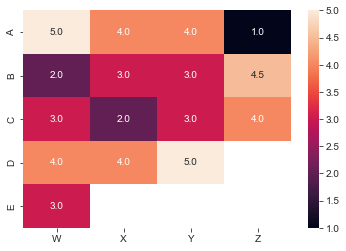
\includegraphics[width=\textwidth-20pt]{book-text/ratings_heatmap.png}

A few natural questions emerge:

\begin{enumerate}
\item What's the most popular cheese? From the observations so far, it's looking like Y is potentially the favorite, but E didn't try Y. 
\item Would D like cheese Z? It seems to be a contentious cheese.
\item If we were asked to buy two cheeses only, which should we buy to satisfy everyone the most?
\end{enumerate}

... and so on. This is cartoonish, and small, but I think the point is clear that this matrix representation above is at least convenient for capturing these ratings.

What may not come obviously is that beyond the convenience of this data visualization, is the mathematical utility of this representation. Question 2 above posits a question that is inherent in the RecSys problem space: "predict how much a user will like an item they've not seen". This question also may be recognizable as a problem from a linear algebra class: "how can we fill in unknown elements of a matrix from the ones we know". This is what is called \emph{matrix completion.}

Before we dive into the linear algebra, let's consider the purely data science perspective called collaborative filtering ([Goldeberg et al, '92](\url{https://d2l.ai/chapter_references/zreferences.html#goldberg-nichols-oki-ea-1992})). The underlying idea is that those with similar taste, help others to know what they like without them having to try it themselves. The collaboration aspect was originally intended to mean among similar-taste users, and the filtering aspect was originally intended to mean filtering out things people wont like.

\section{User-user vs item-item CF}

There are two ways to think of this collaborative filtering strategy:
\begin{itemize}
    \item Two users with similar taste, will continue to have similar taste
    \item Two items with similar user fans, will continue to be popular with other similar users
\end{itemize}

It may sound like these are identical, but perhaps surprisingly, they appear differently in the mathematical interpretations. At a high level, the difference is deciding which kind of similarity do you wish your recommender to make priority of–user similarity or item similarity.

If you prioritize user similarity, then to provide a recommendation for a user $A$, you find a similar user $B$, and then choose a recommendation from $B$'s list of liked content that $A$ hasn't seen  for $A$. 

If you prioritize item similarity, then to provide a recommendation for a user $A$, you find an item that $A$ liked $X$, then you find an item similar to $X$ that $A$ hasn't seen, $Y$, and recommend it for $A$.

Later we will dive deeper into similarity, but let's quickly link these ideas to our brief discussion above. Similar users are rows of the user-item matrix which are similar as vectors; similar items are columns of the user-item matrix which are similar as vectors.


\vspace{10pt}
\colorbox{almond}{\parbox{\textwidth}{
 \emph{Vector similarity} will be more precisely define later, for now, consider similarity to be computed by normalizing the vectors, and then taking their cosine similarity.
}}
\vspace{10pt}


\subsection{The Netflix challenge}

In 2006, an online competition was kicked off on the website \url{www.thenetflixprize.com}. This competition, was to see if teams could improve on the performance of the Netflix team's collaborative filtering algorithms on an open sourced dataset from the company. While this is more common today via websites like Kaggle or via conference competitions, it was very exciting for those interested in RecSys.

The competition consisted of several intermediate rounds of what were called Progress Prize, and the final Netflix Prize was awarded in 2009. The data provided was a collection of 2,817,131 triples consisting of \lstinline{(user, movie, date_rated)}. And half of these additionally include the rating itself. Notice that like our above example, the user-item information is nearly enough to specify the problem. In this particular dataset, the date was provided. Later on, we will dig into how time might be a factor, and in particular, sequential recommendation systems. 

The stakes were quite high in this competition, requirements for beating the internal performance were a 10\% increase in RMSE (we will discuss this loss function later), but the spoils added up to over \$1.1M. The final winners were BellKor's Pragmatic Chaos(who incidentally one the two previous Progress prizes) with a test RMSE of $0.8567$. In the end, only a $20$-min earlier submission kept BellKor ahead of the competitors The Ensemble. 

c.f. 
\begin{itemize}
\item \url{https://www.researchgate.net/publication/223460749_The_BigChaos_Solution_to_the_Netflix_Grand_Prize}

\item \url{https://www2.seas.gwu.edu/~simhaweb/champalg/cf/papers/ProgressPrize2008_BigChaos.pdf}
\end{itemize}
There are a number of important lessons to be learned from this game, but for the sake of brevity:

\begin{itemize}
\item the user-item matrix is at the heart of collaborative filtering and more generally specifying RecSys problems
\item parameter tuning provided a huge improvement in several algorithms
\item several model innovations came from thinking very hard about the business use-case and human behavior
\item linear algebraic approaches served not only as the first reasonably performant solutions, but building on top of them led to the ultimately winning approach
\item eking out the performance that Netflix originally demanded to win the competition too so long, that business circumstances changed, and the [solution was no longer useful]\url{https://thenextweb.com/news/remember-netflixs-1m-algorithm-contest-well-heres-why-it-didnt-use-the-winning-entry}.
\end{itemize}

That last one might be the \lstinline{most} important thing a machine learning developer needs to learn about recommendations systems: build a working usable model quickly and iterate while the business still cares.


\section{Soft ratings}

In our example above, each cheese received either a numerical rating, or was not tried by a guest. These are what are called **hard ratings**–regardless if the cheese is a brie or a chevre; they are explicit, and their absence indicates a lack of interaction between the user and item. In some contexts, we wish to accommodate circumstances wherein a user does interact with an item, and yet no rating is provided.

A common example is a movies app; a user may have watched a movie with the app, but not provided a star rating. This indicates that the item–in this case a movie–has been observed, but we don't have the rating for our algorithms to learn from. However, we can still make use of this implicit data:

\begin{itemize}
\item we can exclude this item from future recommendations
\item we could separately use this data as a separate term in our learner
\item we could assign a default rating value to indicate "interesting enough to watch, not significant enough to rate"
\end{itemize}

It turns out that implicit ratings are very important for training effective recommendation systems, not only because it's common that users don't give hard ratings, but because they provide a different level of signal. Later, when we wish to train multi-level models to predict both click-likelihood and buy-likelihood, these two levels will prove extremely important.

\section{Data collection and user-tracking}

We established above that we learn both from explicit ratings and implicit ratings, so how and where do we get this data? To dive into this, we'll need to start worrying about application code. In many businesses, the data scientists and ML engineers are separate from the engineers, but for recommendation systems, there's a strong need for alignment between the two functions.

\subsection{What to track}

The simplest and most obvious data collection is user-ratings. If users are given the option to provide ratings or even thumbs-up and thumbs-down, that component will need to be built and that data will be stored. These ratings must be stored not only for the opportunity to build recommendations, it's also a bad user experience to rate something and then shortly thereafter the rating doesn't appear if you revisit the page.

Similarly, it's useful to understand a few other key interactions that we will see can improve and expand your RecSys: \lstinline{page loads}, \lstinline{page views}, \lstinline{clicks}, and \lstinline{add-to-bag}.

For these data, let's use a slightly more complicated example, an e-commerce website. Let's take for this example www.bookshop.org. There are many different applications of RecSys on this one page, almost all of which we will return to in time, but for now let's focus on some interactions.

\vspace{10pt}
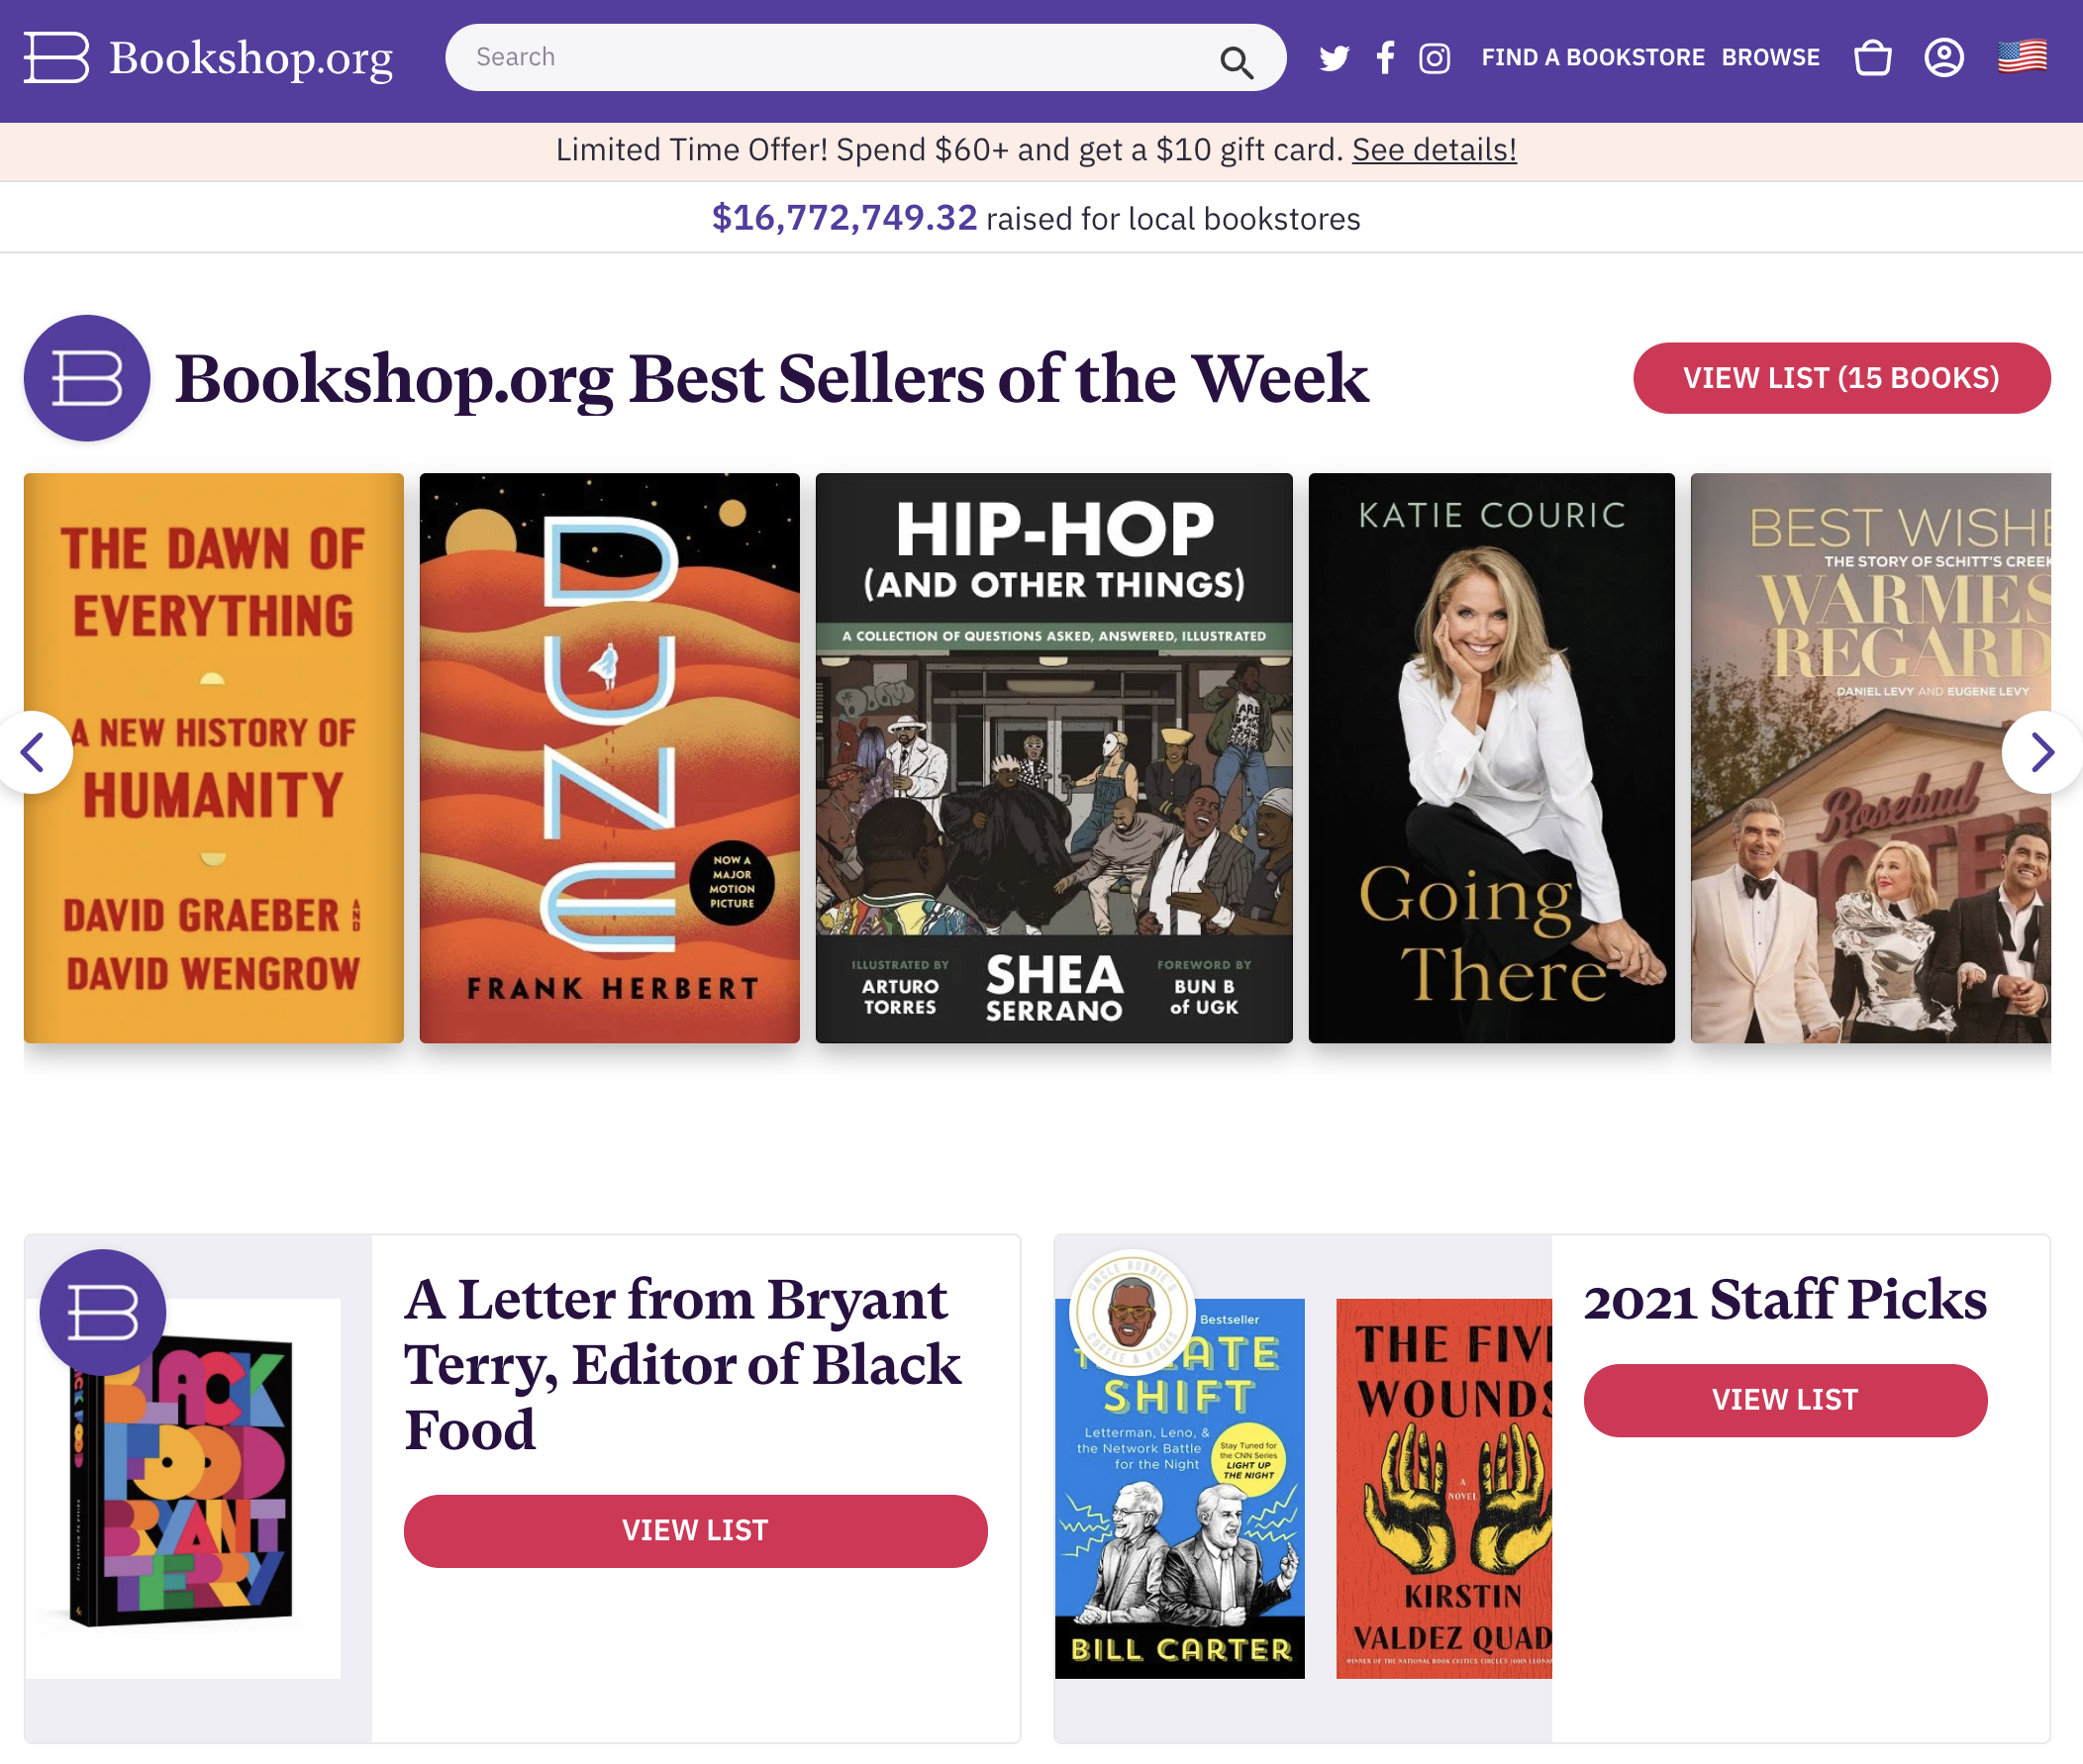
\includegraphics[width=\textwidth-10pt]{book-text/bookshop-landingpage.png}

\paragraph{Page Loads}

When you first load up Bookshop, it starts with items on the page. In the above screenshot, the \emph{Best Sellers of the Week} are all clickable images to those book listings. Despite the user having no choice in this initial page, it's actually quite important to log what is contained in this initial page load. 

These options provide the population of books that the user has seen. If a user has seen an option, then they have the opportunity to click on it, which will ultimately be an important implicit signal. 


\vspace{10pt}
\colorbox{almond}{\parbox{\textwidth}{ This notion is deeply tied to **propensity score matching;** in mathematics, propensity scores are the probability that an observational unit will be assigned to the treatment vs. the control.
}}
\vspace{10pt}

Compare this to the simple 50-50 A/B test: every unit has a 50\% chance of being exposed to your treatment. In a feature-stratified A/B test, you purposely change the probability of exposure dependent on some feature or collection of features (often called covariates in this context). Those probability of exposures are the propensity scores. 

So why bring up A/B testing here? Later, we'll be interested in mining our soft ratings for signal on user preference, but we must consider the possibility that the lack of a soft rating, is not an implicit bad rating. Thinking back to the cheeses: taster D never had a chance to rate Z, so there's no reason to think D has a preference or aversion in Z. This is because D was not **exposed to Z.** Now thinking back to Bookshop: the page above does not show The Hitchhiker's Guide to the Galaxy, so I have no way to click on it, and thus implicitly communicate that I'm interested in that book. I could use the search, but that's a different kind of signal(which we'll talk about later and, in fact, is a much stronger signal).

When understanding implicit ratings like "did the user look at something" we need to properly account for the entire population of things they were exposed to, and use the inverse of that population size to weight the importance of clicking. For this reason, understanding *all* page loads is important.

\paragraph{Page views and hover}

Websites have gotten much more complicated, and now there are a variety of interactions one must contend with. Look what happens if I click the right arrow in the \emph{Best Sellers of the Week} carousel and then move my mouse over the \emph{Cooking at Home} option:


\vspace{10pt}

\includegraphics[width=\textwidth-10pt]{book-text/bookshop-top-sellers.png}

I've unveiled a new option, and mousing over it, made it larger and have a visual effect. These are ways to communicate to the user more information, and remind the user that these are clickable. To the recommender, these can be used as more implicit feedback.

First, the user clicked the carousel scroll–so some of what they saw in the carousel was interesting enough to dig further. Second, they moused over *Cooking at Home* they might click, or they might just want to see if there's additional information when hovering. Many websites use a hover interaction to provide a pop-up detail. While bookshop doesn't implement something like this; internet users have been trained to expect this behavior by all the websites that do, and so the signal is still meaningful. Third, they've now uncovered a new potential item in their carousel scroll–something we should add to our page loads, but really should come with a higher rating because it required interaction to uncover. 

All this and more can be encoded into the website's logging, rich and verbose logging is one of the most important thing to improve a recommendation system, and it's almost always better to have more than you need rather than the opposite.

\paragraph{Clicks}

If you thought hovering meant interest, wait until you hear about clicking! Not in all cases, but in the large majority, clicking is a very strong indicator of product interest. For e-commerce, clicking often is computed as part of the recommendation team's core KPIs (key performance indicators). 

This is for two reasons:

\begin{itemize}
\item clicking is almost always required to purchase; so it's an upstream filter for all business transactions
\item clicking requires explicit user action; so it's a good measure of intent
\end{itemize}

There will always be noise of course, but clicks are the go-to indicator of what a client is interested in. Many production recommendation systems are trained on click data–not ratings data–because of the much higher data volume and because of strong correlation between click behavior and purchase behavior. 


\vspace{10pt}
\colorbox{almond}{\parbox{\textwidth}{ Sometimes in Recommendation Systems you hear people talk about 'click-stream' data. It is an important view into clicks data, that also considers the order of a users click in a single 'session'. Modern recommendation systems put a lot of effort into utilizing the order of items a user clicks on, calling this sequential recommendations, and have show dramatic improvements via this additional dimension. We will discuss sequence-based recs later in the book.
}}
\vspace{10pt}

\paragraph{Add to bag}

We've finally arrived, the user has added some item to their bag or cart or queue. This is an extremely strong indicator of interest, and is often very strongly correlated with purchasing. There are even reasons to argue that add-to-bag is a better signal than purchase/order/watch. Add-to-bag is essentially the end of the line for soft ratings, and usually beyond this you'd want to start collecting ratings and reviews.


\paragraph{Collection and instrumentation}

Web applications very frequently instrument all of the above via 'events'. If you don't yet know what events are, maybe ask a buddy in your engineering org–but we'll give you the skinny. Like logging, events are specially formatted message that the application sends out when a certain block of code is executed. Like in the example of a click, the application needs to make a call to get the next content to show the user. It's common to also "fire an event" at this moment indicating information about the user, what they clicked on, the session id for later reference, the time, and various other useful things. This event can be handled downstream in any number of ways, but there's a increasingly possible pattern of it's path bifurcating to:

\begin{itemize}
\item a log database, like a mysql application database tied to the service
\item an event stream for real-time handling
\end{itemize}

The latter is actually what's interesting to us here. Event streams are often connected up to listeners via technologies like Kafka. This kind of infrastructure can get complicated fast (consult your local data engineer or devOps person), but a simple model for what happens is that all of a particular kind of log are sent to a bunch of different destinations that you think can make use of these events.

In the recommender case, an event stream can be connected up to some transformations to process the data for downstream learning tasks. This will be enormously useful if you want to build a recommendation system that uses those logs. Other important uses are real-time metrics tracking for what's going on at any given time on the website.

\subsection{Aside: Funnels}

We've just worked through our first example of a funnel, and no good Data Scientist can avoid thinking about funnels at some point. Like them or hate them, funnel analyses are crucial for critical analyses of your website, and by extension your recommendation system.


\vspace{10pt}
\colorbox{almond}{\parbox{\textwidth-20pt}{ A \emph{funnel} is a collection of steps a user must take to get from one state to another; it's called a funnel because at each of the discrete steps, a user may stop proceeding through or 'drop off', thus reducing the population size at each step.
}}

\vspace{10pt}
In our discussion of events and user tracking; each step was relevant for a subset of the previous. This means that the process was a funnel, and understanding the drop-off rate at each step, reveals important characteristics of your website, and your recommendations.

\vspace{10pt}
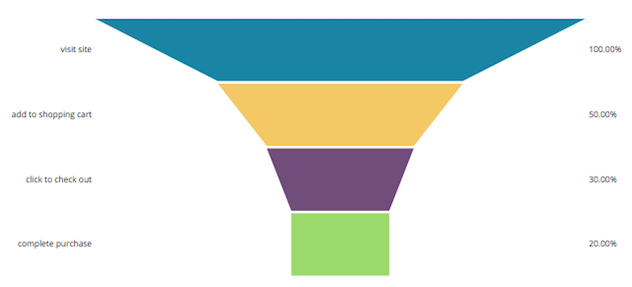
\includegraphics[width=\textwidth-10pt]{book-text/funnel.png}

There are actually three important funnel analyses to be done above:

\begin{itemize}
\item page view to add-to-bag user flow
\item page view to add-to-bag per recommendation
\item add-to-bag to complete purchase
\end{itemize}

The first funnel is merely understanding at a high level, what percentage of users take each step in the above flow. This is a high level measure of your website optimization, the general interestingness of your product offering, and the quality of your user leads.

The second funnel is more fine-grained to take into consideration the recommendations themselves. As mentioned above in the propensity scoring, users can only proceed through the funnel for a particular item if they're shown the item. This intersects with these ideas of funnels because you want to understand at a high level how certain recommendations correlate with funnel drop-off, but also when using a recommender system, the confidence in your recommendations should correlate well with the funnel metrics. We will return to this more in detail later when we discuss loss functions, but for now you should remember to think of different categories of recommendation-user pairs and how their funnels may look compared to average.

Finally, add-to-bag to completion. This actually isn't part of the RecSys problem, but should be on your mind as a Data Scientist or Machine Learning engineer trying to improve the product. **No matter how good your recommendations are, this funnel may destroy any of your hard work.** Before working on a recommender problem, you should almost always investigate the funnel performance in getting a user from add-to-bag to check-out-completed. If there's something cumbersome, or difficult about this flow, it will almost certainly provide a bigger bang-for-your-buck to fix this, than to improve recommendations. Investigate the drop-offs, do user-studies to understand what might be confusing, work with product and engineering to ensure everyone is aligned on this flow before you start building a recommender for e-commerce.

\section{Business insight and what people like}

In the above example from Bookshop.org, we notice that *Top Sellers of the Week* is the primary carousel on the page. Recall our earlier work on \lstinline{get_most_popular_recs}, this is simply that recommender but applied to a specific Collector–one that only looks in the last week. 

This carousel is an example of a recommender providing business-insight, in addition to driving recommendations. A common mission of a growth team is to understand weekly trends and KPIs, often things like weekly-active-users, and new signups. For many digital-first companies, growth teams are additionally interested in understanding the primary drivers.

Let's take an example: as of the writing of this, the Netflix show ***Squid Game*** became Netflix' most popular series of all time, breaking a huge number of records in the process. Squid Game achieved 111 Million viewers in the first month. Most obviously, *Squid Game* needs to be featured in *Top Shows of the Week* or *Hottest Titles* carousels, but what else does a breakout hit like this matter?

The first important insight companies almost always ask for is **attribution**–if the numbers go up in a week, what led to that? Is there something important or special about launches that drove additional growth? How can we learn from that to do better in the future? In the case of *Squid Game*–a foreign-language show that saw massive interest with an English-speaking crowd–executives might take away the inclination to invest more in shows from South Korea, or subtitled shows with high-drama. The flip side of this coin is also important, when growth metrics lag, executives nearly always ask why–being able to point to what was the most popular, and how it may have deviated from expectation, helps a lot.

The other important insight can feed back into recommendations; during exciting debuts like *Squid Game*, it's easy to get caught up in the excitement as you see all your metrics go up and to the right, but might this negatively effect things also? If you have a debut show the same week or two as *Squid Game's* you'll be less enthusiastic about all this success. Overall, successes like this usually drive *incremental* growth which is great for business, and in total, metrics will all probably look up. Other items however may have less successful launches due to a zero-sum game amongst the core user base. This can have a negative effect on longer term metrics, and even can make later recommendations less effective. 

Later, we will learn about diversity of recommendations. There are a large number of reasons to care about diversifying your recommendations, but here we observe one which is to increase the overall matching valence of your users with items. As you keep a broad base of users highly engaged, you increase your future opportunity for growth.

\vspace{10pt}
\colorbox{almond}{\parbox{\textwidth-20pt}{ \emph{Incremental gains} is a term modified from economics and put to use in growth marketing and growth analytics. Incremental gains refer to a margin of increase in addition to the gains expected from an expended effort. A simple example would be a business that usually adds a user for ever \$100 in marketing spend, gets some positive press, and the next week they get a user for every \$80 in marketing spend. If they keep their marketing budget fixed that week at \$1600, they would get 20 new users instead of 16; an incremental gain of 4 users. This is especially common when testing new treatments or programs.
}}

\vspace{10pt}
Finally, beyond surfacing the trending hits, another benefit of knowing what's really hot on your platform or service, is advertising. When a phenomenon starts, there can be a huge advantage in priming the pump, i.e. making noise and publicity of the success. This sometimes leads to a network effect, and in the days with viral content and easy distribution, this can have multiplier effects on your platform's growth.

\chapter{Mathematical Considerations}
\label{ch:math}

\section{Zipf's laws in RecSys and the Matthew Effect}

In a great many applications of machine learning, a caveat is given early, that the distribution of observations of unique items from a large corpus is modeled by Zipf's law. In recommendation systems, the \emph{Matthew Effect} appears in the popular item's click rates, or the popular user's feedback rates. 

Simply, the Matthew Effect–or popularity bias–states that the most popular items continue to attract the most attention and widen the gap with other items. Take for example the MovieLens dataset, an extremely popular dataset for benchmarking recommendation systems[link to MovieLens info], in [[Jenny Sheng 2020]\url{https://jennysheng.com/jenny-sheng-iw-fall-2020.pdf}] they observe the following behavior for number of movie ratings:

\vspace{10pt}
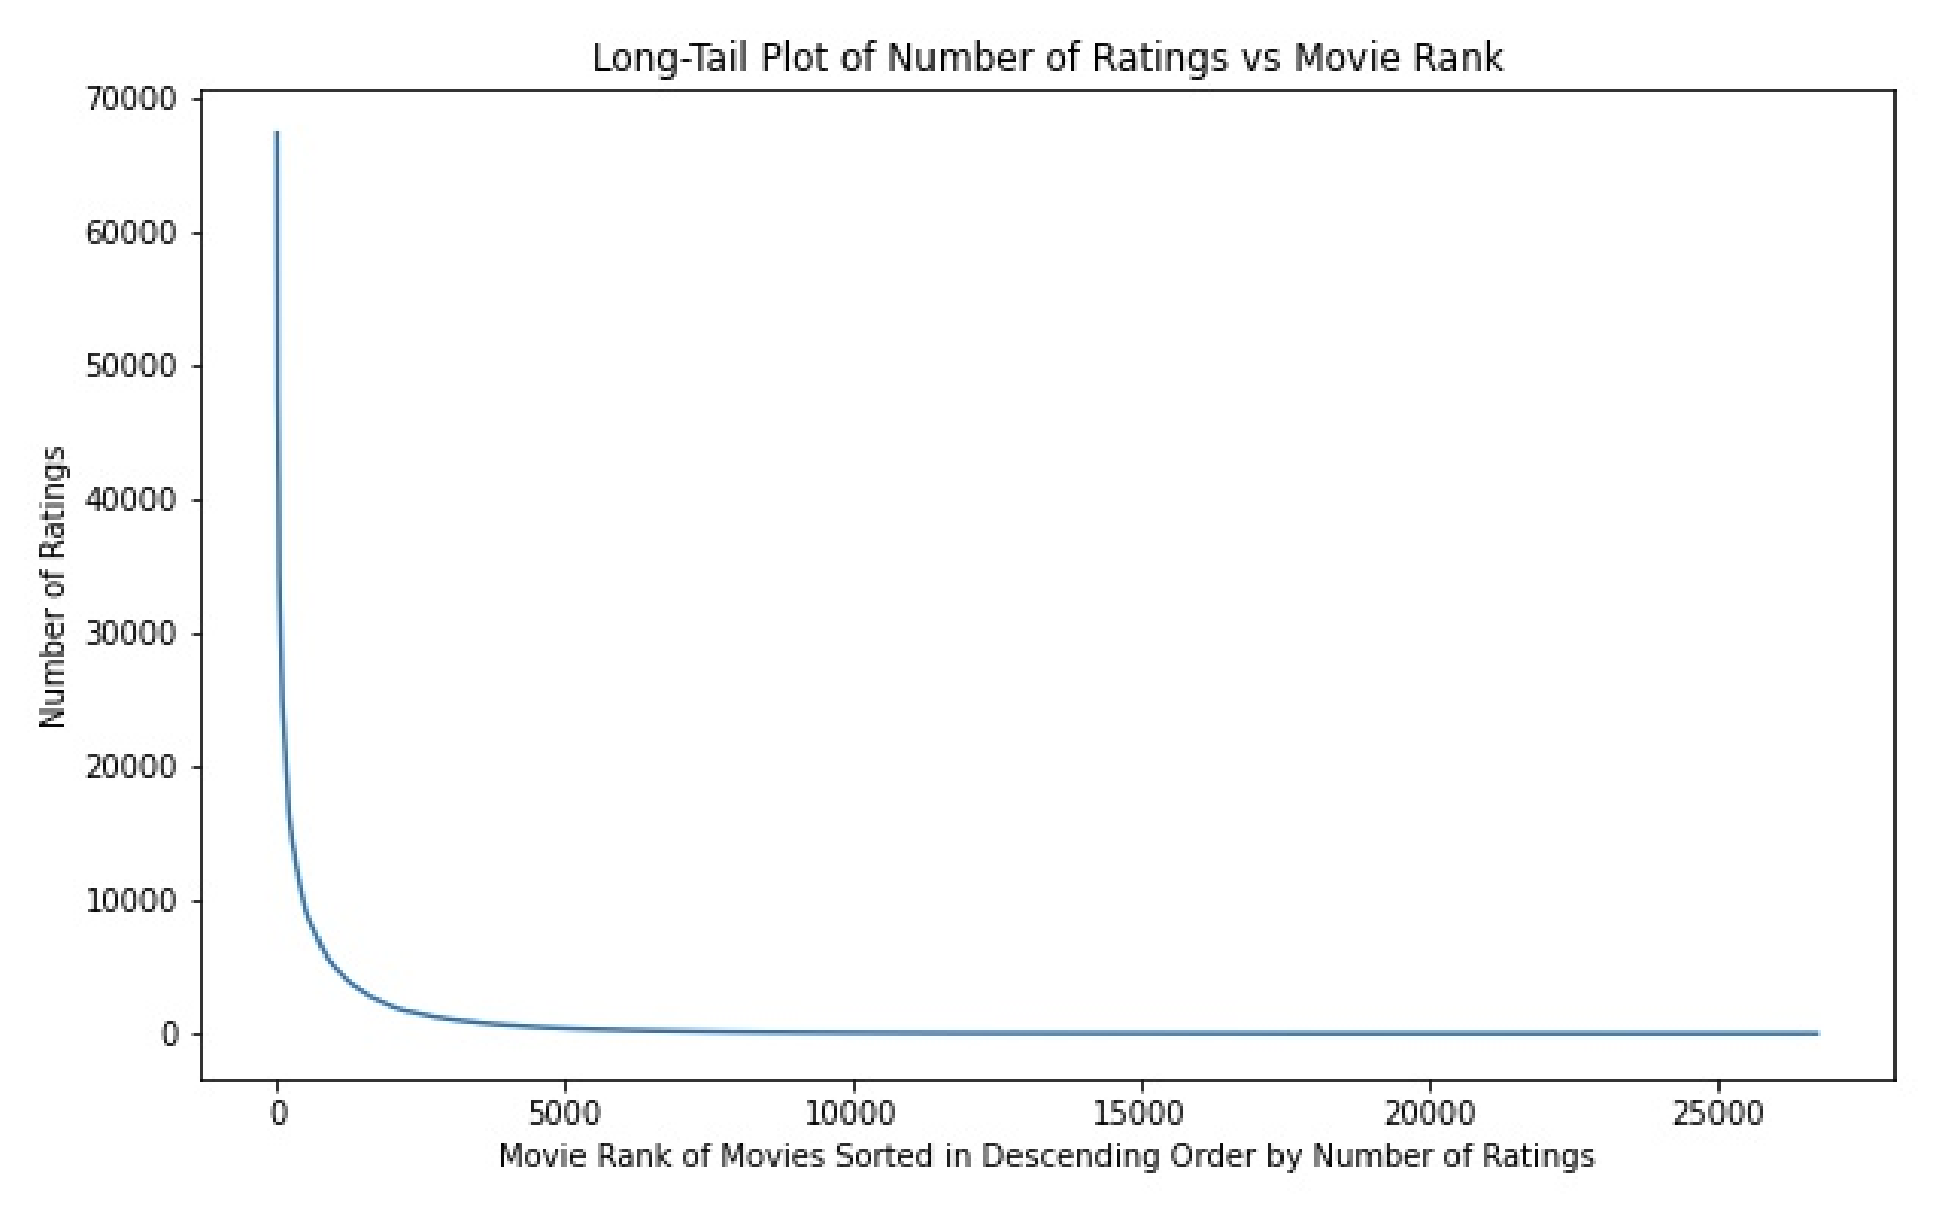
\includegraphics[width=\textwidth-10pt]{book-text/zipfian-moverank.png}

At first glance this behavior is obvious and stark, but is it a problem? Let's assume our recommender will be built as a user-based CF model–as alluded to in \ref{ch:user-item}–then how might these distributions effect the recommender?

Let the probability mass function be described by the simple Zipf's law:

\begin{equation}
    f(k, M) = \frac{1/k}{\sum^M_{n=1}(1/n)}    
\end{equation}


for $M$ number of tokens in the corpus (in the above examples number of movies), $k$ is the rank of a token when sorted by number of occurrences. 

Let's consider users $A$ and $B$, with $N_A = \mathcal{I}_A$  and $N_B = \mathcal{I}_B$ ratings respectively, Observe that the probability of $V_i$, the $i$'th most popular video, appearing in $\mathcal{I}_X$ for some user $X$ is given by:
\begin{equation}
    P(i)=\frac{f(i,M)}{\sum^M_{j=1}f(j,M)}=\frac{1/i}{\sum^M_{j=1}1/j}
\end{equation}

and thus the joint probability of an item appearing in two user's ratings is:

\begin{equation}
  P(i^2)=\left(\frac{1/i}{\sum^M_{j=1}1/j}\right)^2.  
\end{equation}

This becomes important when one also considers that our, yet unstated, definition of user-based collaborative filtering, is based on similarity in user's ratings sets–\emph{number of jointly rated items by two users, divided by the total number of items rated by either.}

Taking this definition, we can for example, compute the similarity score for one shared item amongst $A$ and $B$:

\begin{equation}
    \sum^M_{i=1} \frac{P(i^2)}{\| \mathcal{I}_A \cup \mathcal{I}_B \|},
\end{equation}

and the average similarity score of two users is generalized to:

\begin{equation}
    \sum^{\min(N_A,N_B)}_{t=1}\left(\prod_{i_k=i_{k-1}+1}^{t-1}\sum^M_{i=1} \frac{P({i_k}^2)}{\frac{\| \mathcal{I}_A \cup \mathcal{I}_B \|}{t}}\right).
\end{equation}

These combinatorial formulas indicate not only the relevance of the Zipfian in our algorithms, but we see an almost direct effect on the output of scores. Consider the experiment from [(Wang, Wang, and Zhang 2019)]\url{https://arxiv.org/abs/1909.12798}; for LastFM users, the authors demonstrate average similarity scores for pairs of users, and they find this Matthew Effect persists into the similarity matrix:

\vspace{10pt}
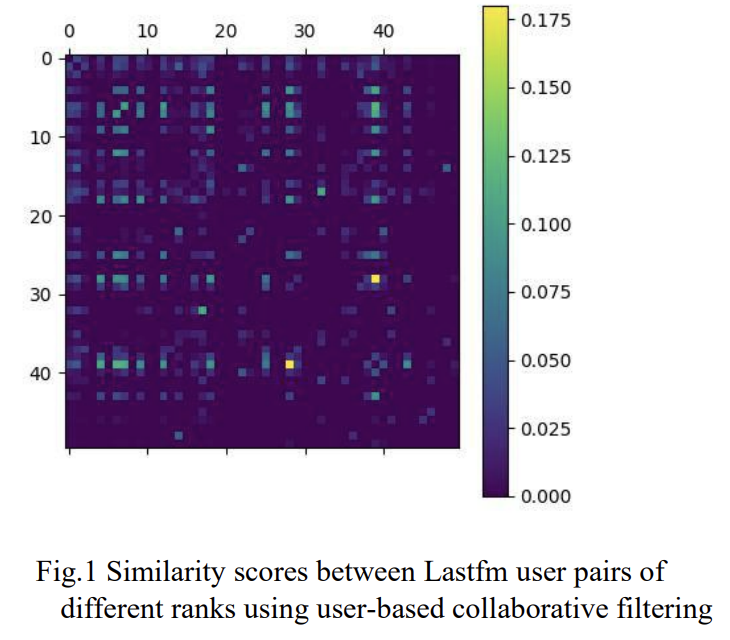
\includegraphics[width=\textwidth-10pt]{book-text/lastfm-matthew-effect.png}

While these results might seem scary, we'll observe later via diversity-aware loss functions that we can mitigate some of this. An even simpler way, is to use downstream sampling methods, which we will discuss as part of our explore-exploit algorithms. Finally, the Matthew Effect is only the first of two major impacts of this Zipfian–let's turn our attention to the second.


\section{Sparsity}

We now must reckon with sparsity. As the ratings skew more and more towards the most popular items, the least popular items a starved for data and recommendations, which is called \emph{Data Sparsity.} This connects to the linear algebraic definition of sparsity, mostly zeros or not populated elements in a vector, when you consider again our user-item matrix less popular items constitute columns with very few entries–these are sparse vectors. Similarly, at scale we see that the Matthew effect pushes more and more of the total ratings into certain columns, and the matrix becomes sparse in the traditional mathematical sense. For this reason, sparsity is an extremely well known challenge for recommendation systems. 

Like above, let's consider the implication on our collaborative filtering algorithms from these sparse ratings. Again observe that the probability of $V_i$, the $i$'th most popular item, appearing in $\mathcal{I}_X$ for some user $X$ is given by:

\begin{equation}
    P(i)=\frac{f(i,M)}{\sum^M_{j=1}f(j,M)}=\frac{1/i}{\sum^M_{j=1}1/j}
\end{equation}

then 

$$(M-1)*P(i)$$

is the expected number of other users which click the $i$'th most popular item, so summing over all $i$ yields the total number of other users that will share a rating with $X$:

\begin{equation}
    \sum_{i=1}^M (M-1)*P(i)
\end{equation}

Again, as we pull back to the overall trends, we observe this sparsity sneaking into the actual computations for our collaborative filtering algorithms, consider the trend of users of different ranks, and how much their rankings are used to 'collaborate' in other user's rankings:

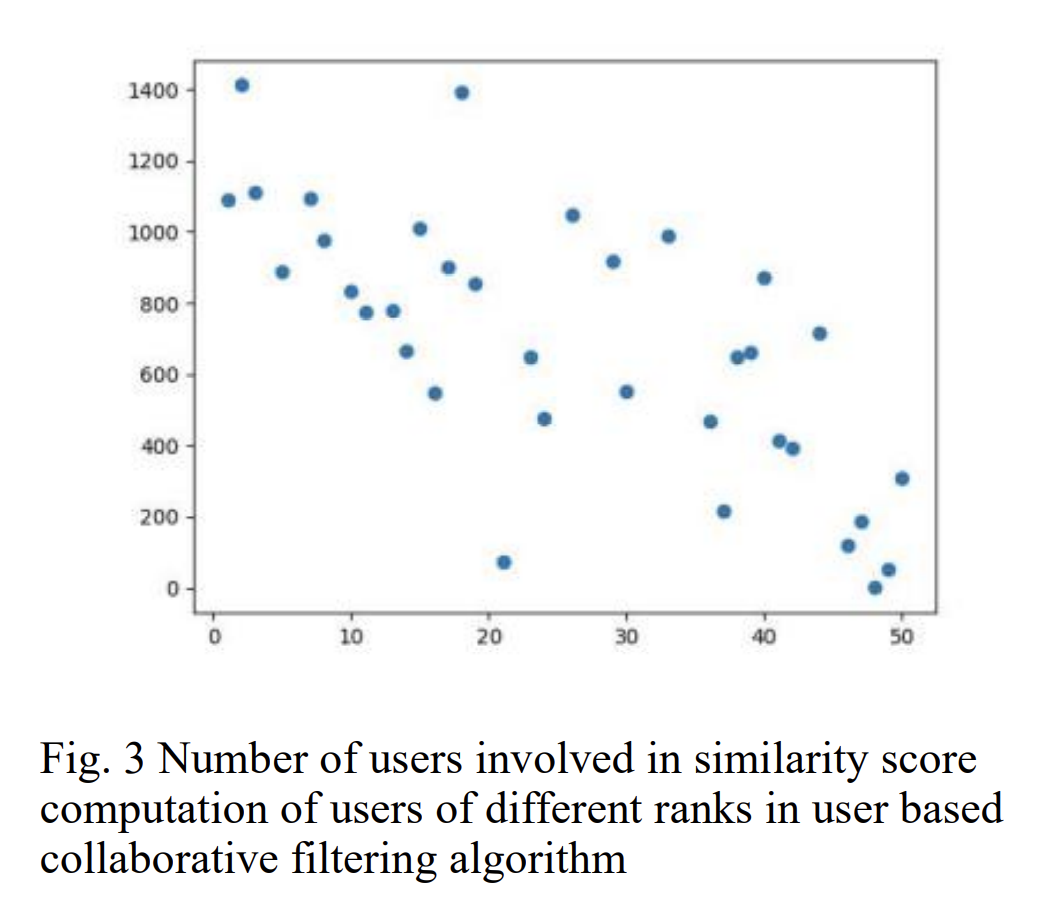
\includegraphics[width=\textwidth-10pt]{book-text/user-sim-counts.png}

We see that this is an important result to always beware–sparsity pushes emphasis onto the most popular users, and has the risk of making your recommender myopic. 

\subsection{Item-based collaborative filtering}

While the equations are different, everything above applies similarly to item-based collaborative filtering. We see similarity in items exhibit the same inheritance of the Zipfian in their scores, and we see items consulted in the collaborative filtering process drops off by rank. 

\section{User Similarity for Collaborative filtering}

In mathematics, it's most common to hear discussion of \emph{distances}–even back to the Pythagorean theorem, we are taught to think of relationships between points as distances, or dissimilarity. Indeed, this fundamental idea is canonized in mathematics as part of the definition of a metric:
\begin{itemize}
    \item $d(a,c)\leq d(a,b)+d(b,c)$
\end{itemize}


In machine learning; we often instead concern ourselves with the notion of similarity–an extremely related topic. In many cases, one can directly pass back and forth between similarity and dissimilarity; when $d:X\times X\rightarrow [0,1]\subset\mathbb{R}$ then we often define:

\begin{equation}
    Sim(a,b):=1-d(a,b)
\end{equation}

This may seem like a needlessly precise statement, but in fact we'll see that there are a [variety of options for how to frame similarity]\url{https://en.m.wikipedia.org/wiki/Similarity_measure}. Furthermore, sometimes we even formulate similarity measures where the associated distance measure does not establish a metric on the set of objects. These so-called pseudo-spaces can still be incredibly important, and we'll see where they come up in the later section on latent spaces. 

In the literature, you'll find a very common practice of papers starting by introducing a new similarity measure, and then training a model you've seen before on the new similarity measure. As we'll see, choices in how you choose to relate objects(users, items, features, etc.) can have a large effect on what your algorithms learn. 

For now, let's laser in on some specific similarity measures. Consider a classic ML problem of clustering; we have a space (usually $\mathbb{R}^n$) in which our data is represented and we are asked to partition our data into sub-collections of the population and assign these collections names. Frequently, these collections are intended to capture some meaning, or at the very least be useful for summarizing the collection elements' features. When you do that clustering, you frequently are considering points near to one another in that space. Further, if you're given a new observation, and asked to assign it to a collection as an inference task you normally compute the new observation's \emph{nearest neighbors}. This could be the k-nearest neighbors, or simply the nearest neighbor amongst cluster centers; either way, your task is to use the notion of similarity to associate. In collaborative filtering, this same notion is used to relate a user for whom you wish to make recommendations, to those you already have data from. 

So how may we define similarity for our users in collaborative filtering? They're not obviously in the same space, so our usual tools seem to be lacking. 

\subsection{Pearson correlation}

Our original formulation of Collaborative Filtering was to say that users with similar taste collaborate to recommend items for each other. Let two users $A$ and $B$, have a set of co-rated items–simply the set of items with ratings from each–written $\mathcal{R}_{A,B}$, and a rating of item $x$ by user $A$ written as $r_{A,x}$, then 

\begin{equation}
    \sum_{x\in \mathcal{R}_{A,B}}(r_{A,x}-\bar{r}_A)
\end{equation}

is the average deviation from $A$'s average rating over all of its co-rated items with $B$. If we think of these ratings as a random variable, and consider the analog for $B$, then the correlation between the jointly distributed variables, i.e. the population covariance, is our \emph{Pearson correlation:}

\begin{equation}
USim_{A,B}=\frac{\sum_{x\in \mathcal{R}_{A,B}}(r_{A,x}-\bar{r}_A)(r_{B,x}-\bar{r}_B)}{\sqrt{\sum_{x\in \mathcal{R}_{A,B}}(r_{A,x}-\bar{r}_A)^2} \sqrt{\sum_{x\in \mathcal{R}_{A,B}}(r_{B,x}-\bar{r}_B)^2}}    
\end{equation}

It's extremely important to keep in mind a few details here:

- This is the similarity of the jointly distributed variables describing the users' ratings
- We compute this via all co-rated items, so user similarity, is defined via item-ratings
- This is a pairwise similarity measure taking values in $[-1,1]\in \mathbb{R}$

\subsection{Ratings via similarity}

Now that we've introduced user-similarity, let's use it!

For a user $A$, and item $x$, we can estimate the rating via similar users' ratings:

\begin{equation}
    Aff_{A,i}=\bar{r}_A+\frac{\sum_{U\in \mathcal{N}(A)}USim_{A,U}*(r_{U,i}-\bar{r}_A)}{\sum_{U\in \mathcal{N}(A)}USim_{A,U}}
\end{equation}

This is the prediction for user $A$'s rating of item $x$, which takes $A$'s average adjusted rating of the similarity-weighted average ratings of all of $A$'s neighbors. In other words: $A$'s rating will probably be the average of people like $A$'s rating, adjusted to how generous $A$ is with ratings in general.

But wait! What's $\mathcal{N}(A)$? It's the neighborhood of $A$, via our $USim$ definition above. How many neighbors? How do you pick those neighbors? These will be the subject of later chapters; for now, assume they're $k$-nearest neighbors and assume some hyperparameter tuning is used to determine a good value for $k$.

\subsection{Fun aside:}

You might wonder, "does this Pearson correlation yield a metric space under some transformation?". The answer is yes, but it's a bit more complicated than our simple definition above. While the above can get us a distance, it's not good enough to get us a metric space, without a more novel transformation.

In particular, for $P(A,B)$ the above defined correlation, then $1-P(A,B)$ yields a distance that satisfies all metric properties *except* the triangle inequality. There are several known ways to adjust this though: $\sqrt{1-P(A,B)^2}$ being the most common. For a survey, see ([Dongen and Enright, 2012]\url{https://arxiv.org/pdf/1208.3145.pdf})

\section{Explore–exploit as a RecSys}

In the previous we saw two ideas, slightly in contrast to one another:

\begin{itemize}
\item The MPIR, a simple easy to understand recommender
\item The Matthew effect in recommendation systems, and it's runaway behavior in distributions of ratings
\end{itemize}

By now, it's likely that you realize that the MPIR will amplify the Matthew effect, and that the Matthew effect will drive the MPIR to the Trivial recommender in the limit. This is the classic difficulty of maximizing a loss function with no randomization–it very quickly settles into a mode.

This problem–and many others like it–encourage some modification to the algorithm to prevent this failure mode, and continue to expose the algorithm and users to other options. The basic strategy for \emph{explore-exploit schemes,} or \emph{multi-armed bandits} as they're called, is to take not only the outcome-maximizing recommendation, but also a collection of alternative \emph{variants,} and randomly determine which to use as response. 

Taking a step back: given a collection of variant recommendations, or \emph{arms}, $A$, for which the outcome of each recommendation is $y_t$, and we have a prior reward function $R(y_t)$. The bandit–called an \emph{agent} in this literature–would like to maximize $R(y_t)$, but the agent doesn't know the distribution of the outcomes $Y_{a\in A}$. The agent thus assumes some prior distributions for $Y_{a\in A}$, and then collects data to update those distributions; after sufficient observations, the agent can estimate the expected values of each distribution, $\mu_{a\in A}=\mathbb{E}(\mathcal{R}(Y_a))$. If the agent was able to confidently estimate these reward values, the recommendation problem would be solved: at inference, the agent would simply estimate the reward values for all variants for the user, and select the reward-optimizing \emph{arm.} This is of course ridiculous in totality, but the basic idea is useful nonetheless: hold prior assumptions about what will be greatest expected reward, and explore alternatives with some frequency to continue to update the distributions and refine your estimators.

\subsection{$\epsilon$-greedy}

So how often should you explore vs. use your reward-optimizing arm? The first best algorithm is $\epsilon$-greedy; for $\epsilon \in (0,1)$, at each request the Agent has probability $\epsilon$ of choosing a random arm and probability $1-\epsilon$ of selecting the currently highest estimated reward arm.

Let's take the MPIR and slightly modify it to include some exploration. 

\begin{lstlisting}[language=Python]
import random

def get_item_popularities() -> Optional[Dict[str, int]]:
	...
		return item_choice_counts # Dict of pairs: (item-identifier, count item chosen)
  return None

def get_most_popular_recs_ep_greedy(
	max_num_recs: int, 
	epsilon: float
) -> Optional[List[str]]:
	assert epsilon<1.0
	assert epsilon>0

	items_popularity_dict = get_item_popularities() # type: Optional[Dict[str, int]]
	if items_popularity_dict:
		sorted_items = sorted(
			items_popularity_dict.items(), 
			key=lambda item: item[1]),
			reverse=True,
		)
		top_items = [i[0] for i in sorted_items]
		recommendations = []
		for i in range(max_num_recs): # we wish to return max_num_recs
			if random.random()>epsilon: # if greater than epsilon, exploit
				recommendations.append(top_items.pop(0))
			else: # otherwise, explore
				explore_choice = random.randint(1,len(top_items))
				recommendations.append(top_items.pop(explore_choice))
		return recommendations
  return None
\end{lstlisting}

The only modification to our MPIR is that now we have two cases for each potential recommendation from our \lstinline{max_num_recs}; if a random probability is less than our $\epsilon$ then we proceed as before and select the most-popular, otherwise we select a random recommendation. 

Note that we're interpreting maximization of reward as selecting most-popular items. This is an important assumption, and as we move into more complicated recommenders, this will be the crucial assumption that we modify to get different algorithms and schemes.

\paragraph{Collector}

The collector here need not change, we still want to get the item popularities first.

\paragraph{Ranker}

The ranker also does not change! We begin by ranking the possible recommendations by popularity.

\paragraph{Server}

If collector and ranker remain the same, then clearly the server is what must be adapted for this new recommender. This is the case, instead of taking the top items to fill \lstinline{max_num_recs} we now utilize our $\epsilon$ to determine at each step if the next recommendation added to our list should be next in line from the ranker, or a random selection. Otherwise, we adhere to the same API schema, and return the same shape of data.

\subsection{What should $\epsilon$ be?}

In the above, $\epsilon$ is a fixed number for the entire call, but what should the value be? This is actually an area of great study and the general wisdom is to start with large $\epsilon$ (to encourage more exploration) and then reduce over time. The rate at which you decrease it, the starting value, and so on, require serious thought and research. Additionally, it can be tied into your prediction loop and be part of the training process.

\section{The NLP-RecSys relationship}

Let's utilize some intuition from a different area of Machine Learning, Natural Language Processing. One of the fundamental models in NLP is word2vec; a sequence–based model for language understanding that utilizes the words which co-occur in sentences together. 

For skipgram-word2vec, the model takes sentences of words, and attempts to learn the implicit meaning of words via their co-occurrence relationships with other words in those sentences. Each pair of co-occurring words, constitutes a sample that is 1-hot encoded and sent into a vocabulary-sized layer of neurons, with a bottleneck layer, and a vocabulary-sized output layer for probabilities that words will occur.

Via this network, we reduce the size of our representation to the bottleneck dimension, and thus find a smaller dimensional representation of all our words than the original corpus-sized 1-hot embedding. The thinking is that similarity of words can now be computed via vector similarity in this new representation space. 

Why is this related to recommendation systems? Well, because if we take the ordered sequence of user-item interactions, e.g. the sequence of movies a user has rated, you can utilize the same idea from word2vec to find item similarity instead of word similarity. In this analogy, the user history is the 'sentence'.

Previously, using our collaborative filtering similarity, we decided that similar users, can help inform what a good recommendation for a user should be. In this model we instead are finding item-item similarity, so instead we assume that items similar to those a user previously liked, they will also like. 

\subsection{Vector search}

We have build a collection of vector representations of our items, and we claim that similarity in this space (often called a latent-space, representation space, or ambient-space) means similarity in 'likeability' to users.

To convert this to a recommendation, consider a user $A$ with a collection of previously liked items $\mathcal{R}_A$, and consider $\mathcal{A}=\lbrace v_x | x\in \mathcal{R}_A\rbrace$ the set of vectors associated to those items in this latent-space. We are looking for a new item $y$ that we think is good for $A$.

One simple way is to take the closest item to the average of those that $A$ likes:

\begin{equation}
	\textrm{argmin}_y\left\lbrace d(v_y,avg(\mathcal{A}))\mid y\in \textrm{Items}\right\rbrace,
\end{equation}

where $d(-,-)$ is a distance function in the latent-space (usually cosine-distance).

This essentially treats all of $A$'s ratings equally and suggests something near those. In practice, this is often fraught. First, you could weight them by rating:

\begin{equation}
	\textrm{argmin}_y\left\lbrace d(v_y,\frac{\sum_{v_x\in\mathcal{A}}r_x}{|\mathcal{R_A}|})\mid y\in \textrm{Items}\right\rbrace,
\end{equation}

which potentially can improve the representativeness of the user feedback in the recommendations. Alternatively, you might find that a user rates movies across a variety of genre and themes. Averaging here will definitely lead to worse results, so maybe you which to simply find recommendations similar to 1 movie the user liked weighted by that rating:

\begin{equation}
	\textrm{argmin}_y\left\lbrace \frac{d(v_y,v_x)}{r_x}\mid y\in \textrm{Items}, v_x\in\mathcal{A}\right\rbrace.
\end{equation}

Finally, you may even want to do this process several times for different items a user liked to get $k$ recommendations:

\begin{equation}
	\textrm{min-}k \left\lbrace \textrm{argmin}_y\left\lbrace \frac{d(v_y,v_x)}{r_x}\mid y\in \textrm{Items}\right\rbrace\mid v_x\in\mathcal{A}\right\rbrace.
\end{equation}

Now we have $k$ recommendations, each is very similar to something that the user has liked, and is weighted by how much they liked it. And this approach only utilized an implicit geometry of the items formed by their co-occurrences. 

Latent-spaces and the geometric power that comes with them for recommendations will be a through-line for the rest of the book. We will often formulate our loss functions via these geometries, and exploit the geometric intuition to brainstorm where to expand our technique next. 

\subsection{Aside: Nearest-neighbors search}

A reasonable question to ask is "how do I get these vectors that minimize this distance"? In all of the above schemes, we are computing many distances and then finding minimums. In general, the problem of nearest-neighbors is an extremely important and well studied question. While finding the exact nearest-neighbors can sometimes be very slow; a lot of great progress has been made on Approximate Nearest Neighbors search. These algorithms not only return very close to the actual nearest-neighbors, but they perform orders of complexity faster. In general, when you see us (or in many papers) computing an $\textrm{argmin}$ over some distances, there's a good chance approximate nearest neighbors is what's used in practice.



In this section, let's begin our discussion of the core elements of a system that is needed to serve recommendations at industrial scale. In theory, a recommendation system is a collection of math formulae which can take historical data about user-item interactions, and return probability estimates for user-item pair's affinity. In practice, a recommendation system is 5, 10, maybe 20 software systems, communicating in real-time, working with limited information, restricted item-availability, and perpetually-out-of-sample behavior, to ensure the user sees \textit{something.}

This section is heavily influenced by the writing of Karl Higley and Eugene Yan.

\section{Online vs Offline}

In Machine Learning systems, the most frequent terminologies you'll encounter for the two sides of this paradigm are \emph{batch} and \emph{real-time}.
A \emph{batch process} is something that does not require user input, often has longer expected time periods for completion, and is able to have all the necessary data available simultaneously. Batch processes often include things like training a model on historical data, augmenting one data set with an additional collection of features, or computationally expensive data transformation. Another characteristic you see more in batch processes are that it works with the full dataset involved, not only a subset of the data sliced by time or otherwise.

A \emph{real-time} \emph{process} is characterized by something that is carried out at time of request, or said differently, something that is evaluated during the inference process. Examples include: providing a recommendation upon page load, updating 'next episode' after the user finishes the last, re-ranking recommendations after one has been marked 'not interesting'. Real-time processes are often resource-constrained because of the need for rapidity, but like many things in this domain, as the world's computational resources expand, we change the definition of resource-constrained.

Let's return to the previously introduced components–collector, ranker, server–and let's consider their roles in offline and online components. Recall:

\section{Collector}

The collector's role is to know what is in the collection of things that may be recommended, and the necessary features or attributes of those things.

\subsection{Offline Collector}

The offline collector has access to, and is responsible for the largest data sets. Understanding all user-item interactions, user-similarities, item-similarities, feature stores for users and items, and building indices for nearest neighbor lookup are all under the purview of the offline collector.

It's important to remember that the offline collector needs not only access and knowledge of these datasets, but also will be responsible for writing the necessary downstream datasets to be used in real time.

\subsection{Online Collector}

The online collector uses the information indexed and prepared by the offline collector, to provide real-time access to the parts of this data necessary for inference. This includes things like searching for nearest neighbors, augmenting an observation with features from a feature store, or full inventory catalog knowledge. 

One additional role the online collector may take on is encoding a request. In the context of a search recommender, we wish to take the query, and encode it into the 'search space' via an embedding model. For contextual recommenders, we need to encode the context into the 'latent space' via an embedding model also. 

\section{Ranker}

The ranker's role is to take the collection provided by the collector, and order some or all of them, according to a model for the context and user. The ranker actually gets two components itself, the \emph{filtering} and the \emph{scoring.}

Filtering can be thought of as the coarse inclusion and exclusion of items appropriate for recommendation. Usually characterized by rapidly cutting away a lot of potential recommendations that we definitely don't wish to show. A trivial example is not recommending items we know the user has already chosen in the past.

Scoring is the more traditional understanding of ranking: creating an ordering on potential recommendations with respect to the chosen objective function.

\subsection{Offline Ranker}

The offline ranker's goal is to facilitate filtering and scoring. An Important technology that will be discussed later is the \emph{Bloom Filter}. A bloom filter allows the offline ranker to do work in batch, so that filtering in real-time may happen much faster. An over simplification of this process would be to use a few features of the request to quickly select between subsets of all possible candidates; if this step can be made fast–in terms of computational complexity, and striving for something less than quadratic in the number of candidates–downstream complex algorithms can be made much more performant.

Second to the filtering step is the ranking step. In the offline component, ranking is training the model that learns how to rank items. As we will see later, learning to rank items to perform best with respect to the objective function, is at the heart of the recommendation models. Training these models, and preparing the aspects of their output, is part of the batch responsibility of the Ranker.

\subsection{Online Ranker}

The online ranker get's a lot of praise, but really utilizes the hard work of other components. The online ranker first does filtering, utilizing the filtering infrastructure built offline–for example an index lookup or a bloom filter application. After filtering, the number of candidate recommendations has been tamed, and thus we can actually come to the point: rank recommendations.

In the online ranking phase, usually a feature store is accessed to take the candidates and embellish them with the necessary details, and then a scoring and ranking model is applied. Scoring or ranking may happen in several independent dimensions, and then be collated into one final ranking. In the multi-objective paradigm, you may have several of these ranks associated to the list of candidates returned by a ranker.

\section{Server}

The server's role is to take the ordered subset provided by the ranker, ensure that the necessary data schema is satisfied–including essential business logic–and return the requested number of recommendations. 

\subsection{Offline Server}

The offline server is responsible for high level establishment of what are the hard requirements of recommendations returned from the system. In addition to establishing and enforcing schema, this can be more nuanced things like "never return this pair of pants when also recommending this top". Often waved off as "business logic"–the offline server is responsible for creating efficient ways to impose top level priorities on the returned recommendations. 

An additional responsibility for the offline server is handling things like experimentation. There's a good chance at some point you'll want to run online experiments to test out all the amazing recommendation systems you build with this book. The offline server is the place where you'll implement the logic necessary to take experimentation decisions, and provide the implications in a way the online server can use them in real time.

\subsection{Online Server}

The online server takes the rules, requirements, and configurations established, and makes their final application to the ranked recommendations. A simple example would be diversification rules; as we will see later, diversification of recommendations can have a significant impact on the quality of a user's experience. The online server can read the diversification requirements from the offline server, and apply them to the ranked list to return the expected number of diverse recommendations.

It's important to remember that the online server is the endpoint that other systems will be getting a response from. While it's usually where the message is coming from, much of the most complicated components in the system are upstream. Be careful to instrument this system in a way that when responses are slow, each system is observable enough that you can identify where those performance degradations are coming from.

\chapter{System Design for Recommendation System}
\label{ch:system_design}

In this section, let's begin our discussion of the core elements of a system that is needed to serve recommendations at industrial scale. In theory, a recommendation system is a collection of math formulae which can take historical data about user-item interactions, and return probability estimates for user-item pair's affinity. In practice, a recommendation system is 5, 10, maybe 20 software systems, communicating in real-time, working with limited information, restricted item-availability, and perpetually-out-of-sample behavior, to ensure the user sees \emph{something.}

This section is heavily influenced by the writing of Karl Higley, Even Oldridge, and Eugene Yan.

\section{Online vs Offline}

In Machine Learning systems, the most frequent terminologies you'll encounter for the two sides of this paradigm are \emph{batch} and \emph{real-time.}
A \emph{batch process} is something that does not require user input, often has longer expected time periods for completion, and is able to have all the necessary data available simultaneously. Batch processes often include things like training a model on historical data, augmenting one data set with an additional collection of features, or computationally expensive data transformation. Another characteristic you see more in batch processes are that it works with the full dataset involved, not only a subset of the data sliced by time or otherwise.

A \emph{real-time} \emph{process} is characterized by something that is carried out at time of request, or said differently, something that is evaluated during the inference process. Examples include: providing a recommendation upon page load, updating 'next episode' after the user finishes the last, re-ranking recommendations after one has been marked 'not interesting'. Real-time processes are often resource-constrained because of the need for rapidity, but like many things in this domain, as the world's computational resources expand, we change the definition of resource-constrained.

Let's return to the previously introduced components–collector, ranker, server–and let's consider their roles in offline and online components. Recall the components introduced before:

\section{Collector}

The collector's role is to know what is in the collection of things that may be recommended, and the necessary features or attributes of those things.

\subsection{Offline Collector}

The offline collector has access to, and is responsible for the largest data sets. Understanding all user-item interactions, user-similarities, item-similarities, feature stores for users and items, and building indices for nearest neighbor lookup are all under the purview of the offline collector.

It's important to remember that the offline collector needs not only access and knowledge of these datasets, but also will be responsible for writing the necessary downstream datasets to be used in real time.

\subsection{Online Collector}

The online collector uses the information indexed and prepared by the offline collector, to provide real-time access to the parts of this data necessary for inference. This includes things like searching for nearest neighbors, augmenting an observation with features from a feature store, or full inventory catalog knowledge. 

One additional role the online collector may take on is encoding a request. In the context of a search recommender, we wish to take the query, and encode it into the 'search space' via an embedding model. For contextual recommenders, we need to encode the context into the 'latent space' via an embedding model also. 

\section{Ranker}

The ranker's role is to take the collection provided by the collector, and order some or all of them, according to a model for the context and user. The ranker actually gets two components itself, the \emph{filtering} and the \emph{scoring.}

Filtering can be thought of as the coarse inclusion and exclusion of items appropriate for recommendation. Usually characterized by rapidly cutting away a lot of potential recommendations that we definitely don't wish to show. A trivial example is not recommending items we know the user has already chosen in the past.

Scoring is the more traditional understanding of ranking: creating an ordering on potential recommendations with respect to the chosen objective function.

\subsection{Offline Ranker}

The offline ranker's goal is to facilitate filtering and scoring. An Important technology that will be discussed later is the \emph{Bloom Filter.} A bloom filter allows the offline ranker to do work in batch, so that filtering in real-time may happen much faster. An over simplification of this process would be to use a few features of the request to quickly select between subsets of all possible candidates; if this step can be made fast–in terms of computational complexity, and striving for something less than quadratic in the number of candidates–downstream complex algorithms can be made much more performant.

Second to the filtering step is the ranking step. In the offline component, ranking is training the model that learns how to rank items. As we will see later, learning to rank items to perform best with respect to the objective function, is at the heart of the recommendation models. Training these models, and preparing the aspects of their output, is part of the batch responsibility of the Ranker.

\subsection{Online Ranker}

The online ranker gets a lot of praise, but really utilizes the hard work of other components. The online ranker first does filtering, utilizing the filtering infrastructure built offline–for example an index lookup or a bloom filter application. After filtering, the number of candidate recommendations has been tamed, and thus we can actually come to the point: rank recommendations.

In the online ranking phase, usually a feature store is accessed to take the candidates and embellish them with the necessary details, and then a scoring and ranking model is applied. Scoring or ranking may happen in several independent dimensions, and then be collated into one final ranking. In the multi-objective paradigm, you may have several of these ranks associated to the list of candidates returned by a ranker.

\section{Server}

The server's role is to take the ordered subset provided by the ranker, ensure that the necessary data schema is satisfied–including essential business logic–and return the requested number of recommendations. 

\subsection{Offline Server}

The offline server is responsible for high level establishment of what are the hard requirements of recommendations returned from the system. In addition to establishing and enforcing schema, this can be more nuanced things like "never return this pair of pants when also recommending this top". Often waved off as "business logic"–the offline server is responsible for creating efficient ways to impose top level priorities on the returned recommendations. 

An additional responsibility for the offline server is handling things like experimentation. There's a good chance at some point you'll want to run online experiments to test out all the amazing recommendation systems you build with this book. The offline server is the place where you'll implement the logic necessary to take experimentation decisions, and provide the implications in a way the online server can use them in real time.

\subsection{Online Server}

The online server takes the rules, requirements, and configurations established, and makes their final application to the ranked recommendations. A simple example would be diversification rules; as we will see later, diversification of recommendations can have a significant impact on the quality of a user's experience. The online server can read the diversification requirements from the offline server, and apply them to the ranked list to return the expected number of diverse recommendations.

It's important to remember that the online server is the endpoint that other systems will be getting a response from. While it's usually where the message is coming from, much of the most complicated components in the system are upstream. Be careful to instrument this system in a way that when responses are slow, each system is observable enough that you can identify where those performance degradation are coming from.

\part{Retrieval}

\emph{“How do we get all the data in the right place to train a recommendation system, and for real-time inference?”}

Reading research papers in recommendation systems will often give the impression that they’re built via a bunch of math equations, and all the really hard work of recommendation systems is connecting these equations to the features of your problem. More realistically, the first several steps of building a production recommendation system is systems engineering. Understanding how your data will make it into your system, be manipulated into the correct structure, then available in each of the relevant steps of the training flow often constitutes the bulk of the initial recommendation systems work. But even beyond this initial phase, ensuring all of the necessary components are fast enough and robust enough for production environments, requires yet another significant investment in platform infrastructure.

Just in case you’re thinking “I’m a data scientist! I don’t need to know all this!”; RecSys has an inconvenient duality, when the model architecture changes, often so too does the systems architecture. Wanna try out those fancy transformers? Your deployment strategy is going to need a new design. Maybe your clever feature embeddings can solve the cold-start problem! Prepare to serve your encoding layers and integrate with your new NoSql feature store. Don’t panic! This chapter is a walk through the Big Data Zoo.

\chapter{Data Processing}
\label{ch:data-processing}

In the trivial recommender that we introduced in the introduction, we used a method \lstinline{get_availability} and in the MPIR, we used a method \lstinline{get_item_popularities}. We glossed over the details of these two functions, and hoped the choice of naming would provide sufficient context about what their function was. 

Now we wish to start unpacking the details of some of this complexity, and see what the toolsets are for online and offline collectors.

\section{Hydrating your system}

\subsection{PySpark}

Spark is an extremely general computing library, with APIs for Java, Python, SQL, and Scala. PySpark's role in many ML pipelines is for data processing and transformation of the largest scale datasets in your pipeline. 

Recall that the user-item matrix is the linear-algebraic representation of all of the triples of users, items, and the user's rating of the item. These triples are not naturally occurring in the wild–most commonly, you begin with log files from your system:

\begin{lstlisting}[language=python]
{
	'page_view_id': 'd15220a8e9a8e488162af3120b4396a9ca1', 
	'anonymous_id': 'e455d516-3c08-4b6f-ab12-77f930e2661f', 
	'view_tstamp': 2020-10-29 17:44:41+00:00, 
	'page_url': 'https://bookshop.org/lists/bookshop-org-best-sellers-of-the-week', 
	'page_url_host': 'bookshop.org', 
	'page_url_path': '/lists/bookshop-org-best-sellers-of-the-week', 
	'page_title': 'Best Sellers of the Week', 
	'page_url_query': None, 
	'authenticated_user_id': 15822493.0, 
	'url_report_id': 511629659.0, 
	'is_profile_page': False, 
	'product_viewed': 'list', 
}
\end{lstlisting}

These are the kinds of events that you consume from Engineering, and are likely stored in your columnar database. For data like these, utilizing SQL syntax will be our entry point.

PySpark provides a convenient SQL api, and based on your infrastructure, will allow you to write what looks like SQL queries against a potentially massive dataset:

\begin{lstlisting}[language=Python]
user_item_view_counts_qry = """
SELECT 
  page_views.authenticated_user_id
  , page_views.page_url_path
  , COUNT(DISTINCT page_views.page_view_id) AS count_views 

FROM prod.page_views
JOIN prod.dim_users 
	ON page_views.authenticated_user_id = dim_users.authenticated_user_id 

WHERE DATE page_views.view_tstamp >= '2017-01-01'
	AND dim_users.country_code = 'US'

GROUP BY 
	page_views.authenticated_user_id
  , page_views.page_url_path

ORDER BY 3, page_views.authenticated_user_id
"""

user_item_view_counts_sdf = spark.sql(user_item_view_counts_qry)
\end{lstlisting}

Here is a simply SQL query assuming the log schema above, that would allow you to see for each user-item pair, how many times that user has viewed that pair. The convenience of writing pure SQL here means that we can use our experience in columnar databases to quickly ramp up on Spark. The major advantage of Spark, however, is not yet on display. When executing the above in a Spark Session, this query will not be immediately run. This query will be staged for execution, but Spark waits until you use this data downstream in a way that \emph{requires immediate execution} before it begins doing so. This is called lazy-evaluation, and it allows you to work on your data object without every change and interaction immediately being applied. I'll refer you to more serious treatments of Spark for details, but there's one more important characteristic of the Spark paradigm that is essential to discuss.

Spark is natively a distributed computing language. In particular, this means that the above query, even after I force it to execute, will store its data on multiple computers. Spark works via a \emph{driver program} in your program or notebook, which drives a \emph{cluster manager}, which in turn coordinates \emph{executors} on \emph{worker nodes.} When I query data with Spark, instead of all of that data being returned into a DataFrame in memory on the computer I'm using, parts of that data are sent to memory on the executors. And when I do some transformation on the DataFrame, it is applied appropriately on the pieces of the DataFrame that are stored on each of the executors. If this sounds a bit like magic, that's because it is. Spark is a layer of technology that allows the ML Engineer to program as if they're working on one machine, and have those changes take effect on an entire cluster of machines. 

It's important to caveat that all of this does not come for free; both lazy-evaluation and distributed DataFrames come at a cost of needing additional thought when writing programs. Even though Spark makes a lot of this work far easier, understanding how to write efficient code in this paradigm that works with the architecture but still achieves complicated goals, can require a career's worth of experience. 

Returning to Recommendation Systems, and in particular the offline Collector, we want to use PySpark to build the types of data sets needed to train our models. One simple thing you may wish to do with PySpark is the above: transform your logs data into the appropriate form for training a model. In our simple query above, we applied a few filters to our data, and grouped by user and item to get number of views. There are a variety of other tasks that may fit naturally into this paradigm; perhaps adding user or item features stored in other databases, or high-level aggregations.

In our MPIR, we asked for \lstinline{get_item_popularities}, and we sorta assumed a few things:

\begin{itemize}
\item this would return the count of each item's times being chosen
\item this method would be fast
\end{itemize}

The second point is important if this is going to be called in real time. So how might Spark come into play?

First, let's assume we have a lot of data, enough that I can't get it all to fit into my little MacBook Pro's memory. Additionally, let's continue to use the above schema. We can write an even simpler query:

\begin{lstlisting}[language=Python]
item_popularity_qry = """
SELECT 
  page_views.page_url_path
  , COUNT(DISTINCT page_views.authenticated_user_id) AS count_viewers 

FROM prod.page_views
JOIN prod.dim_users 
	ON page_views.authenticated_user_id = dim_users.authenticated_user_id 

WHERE DATE page_views.view_tstamp >= '2017-01-01'
	AND dim_users.country_code = 'US'

GROUP BY 
	page_views.page_url_path

ORDER BY 2
"""

item_view_counts_sdf = spark.sql(item_popularity_qry)
\end{lstlisting}

We can now write this aggregated list of \lstinline{(item, count)} pairs to an app database to serve \lstinline{get_item_popularities}, something that doesn't require us to do any parsing when this is called, or potentially we can take some subset of the top-$N$ of this list and store it in memory. Either way, we've separated concerns of parsing all of our log data, and doing aggregation, from the \lstinline{get_item_popularities} function call in real-time. 

This example used an overly-simple data aggregation, one just as easy to do in something like PostgreSQL, so why bother? The first reason is scalability. Spark is really built to scale horizontally, which means that as the data we need to access grows, we merely add more and more worker nodes. The second reason is that PySpark is more than just SparkSql; anyone who's  done complicated SQL queries can probably agree that the power and flexibility of SQL is enormous, but frequently certain tasks you want to achieve require a lot of creativity to carry out in the fully SQL environment. PySpark gives you all the expressiveness of Pandas DataFrames, Python functions and classes, and a simple interface to apply Python code to the PySpark data structures\textemdash\emph{UDF}s. UDFs are similar to lambda functions that you'd use in Pandas, but they're built and optimized for PySpark DataFrames. As you've probably experienced when writing Machine Learning programs in smaller data regimes, at some point you switch away from only using SQL to using Pandas API functions to perform data transformations–so too will you appreciate this power at the Spark data scale.

PySpark allows you to write what looks very much like Python and Pandas code, and have that code executed in a distributed fashion! You don't need to write code to say on which worker nodes operations should happen, that's handled for you by PySpark. This framework isn't perfect; some things you expect to work may require a bit of care, and optimization of your code can require an additional level of abstraction, but generally PySpark gives you a rapid way to move your code from one node to a cluster and utilize that power.

To illustrate something a bit more useful in PySpark, let's return to Collaborative Filtering, and compute some relevant features.

\paragraph{Example: User similarity in PySpark}

An example of a PySpark job that you might see as part of the Offline Collector's responsibility, would be to build a user-similarity table. Even though in many cases ratings would continue to stream in all the time, for the purposes of large offline jobs we very often think of a daily batch to update the essential tables for our model. In practice, in many cases this daily batch job suffices to provide good enough features for most of the Machine Learning work downstream. While counterexamples exist, even when they do the strategy tends to be how to \emph{marry} the more frequent updates with these daily batch jobs, not how to eliminate them totally. This architecture of daily batch jobs, with smaller more frequent batch jobs is called the \emph{lambda architecture} and we'll get more into the details of how and why later. Note that for the speed layer one may have varying frequencies associated to it. It's possible to have different speed layers for hourly, and another speed layer for minute-frequency jobs that do different things.

 
\begin{figure}[h!]
    \caption{https://hazelcast.com/glossary/lambda-architecture/}
    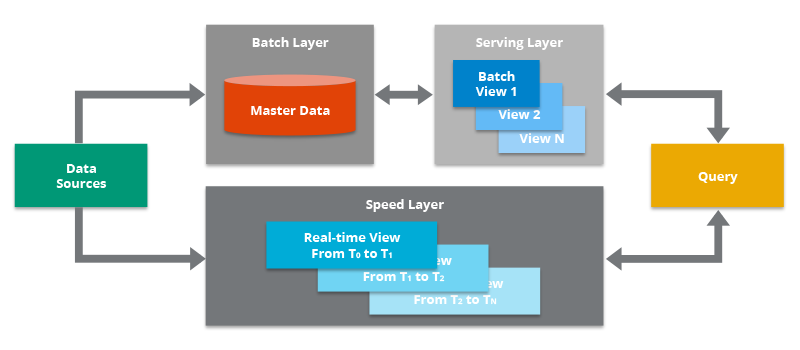
\includegraphics[width=\textwidth-10pt]{book-text/spark-architecture.png}
\end{figure}


In the case of user-similarity, let's work on a batch job implementation of computing a daily table; so first we'll need to get ratings from our schema before today, we also include a few other filters that simulate how this query might look in real life:

\begin{lstlisting}[language=Python]
user_item_ratings_qry = """
SELECT 
  book_ratings.book_id
  book_ratings.user_id
  , book_ratings.rating_value
  , book_ratings.rating_tstamp

FROM prod.book_ratings
JOIN prod.dim_users 
	ON book_ratings.user_id = dim_users.user_id 
JOIN prod.dim_books
	ON book_ratings.book_id = dim_books.dim_books

WHERE 
	DATE book_ratings.rating_tstamp 
		BETWEEN (DATE '2017-01-01') AND (CAST(current_timestamp() as DATE)
  AND book_ratings.rating_value IS NOT NULL
	AND dim_users.country_code = 'US'
  AND dim_books.book_active 
"""

user_item_ratings_sdf = spark.sql(user_item_ratings_qry)
\end{lstlisting}

As before, utilizing the SQL syntax to get the dataset into a Spark DataFrame is the first step, but now we have some additional work on the PySpark side. This is usually the pattern: get the dataset you want to work with via simple SQL syntax and logic, then use PySpark API to do some more detailed data processing.

Let's first observe that we have no assumptions about uniqueness in the above. For the sake of this table, let's decide that we'll use the most recent rating for a pair.

\begin{lstlisting}[language=Python]
from pyspark.sql.window import Window

windows = Window().partitionBy(
	['book_id', 'user_id']
).orderBy(
	col("rating_tstamp").desc()
)

user_item_ratings_sdf.withColumn(
	"current_rating", 
	first(
		user_item_ratings_sdf("rating_tstamp")
	).over(windows).as("max_rating_tstamp")
).filter("rating_tstamp = max_rating_tstamp")
\end{lstlisting}

We'll now use \lstinline{current_rating} as our ratings column for the purpose of downstream calculation.

Recall from before our ratings-based definition of user-similarity: 

\begin{equation}
\mathrm{USim}_{A,B}=\frac{\sum_{x\in \mathcal{R}_{A,B}}(r_{A,x}-\bar{r}_A)(r_{B,x}-\bar{r}_B)}{\sqrt{\sum_{x\in \mathcal{R}_{A,B}}(r_{A,x}-\bar{r}_A)^2} \sqrt{\sum_{x\in \mathcal{R}_{A,B}}(r_{B,x}-\bar{r}_B)^2}}    
\end{equation}



The important values we'll need are:

\begin{itemize}
\item $r_{(-,-)}$
\item $\bar{r}_{(-)}$
\end{itemize}

The rows are already the $r_{(-,-)}$ values, so let's compute user average ratings, $\bar{r}_{(-)}$ and the rating deviations:

\begin{lstlisting}[language=Python]
from pyspark.sql.window import Window
from pyspark.sql import functions as F

user_partition = Window.partitionBy('user_id')

user_item_ratings_sdf = user_item_ratings_sdf.withColumn(
	"user_average_rating", 
	F.avg("current_rating").over(user_partition)
)

user_item_ratings_sdf = user_item_ratings_sdf.withColumn(
	"rating_deviation_from_user_mean", 
	F.col("current_rating") - F.col("user_average_rating")
)
\end{lstlisting}

Now our schema should look like this (formatted slightly nicer than the default spark output):

\begin{lstlisting}[language=Python]
+-------+-------+------------+-------------+
|book_id|user_id|rating_value|rating_tstamp|
+-------+-------+------------+-------------+
+-------------+-------------------+-------------------------------+
current_rating|user_average_rating|rating_deviation_from_user_mean|
+-------------+-------------------+-------------------------------+
\end{lstlisting}

Let's finish creating a dataset that contains our User Similarity calculations:

\begin{lstlisting}[language=Python]
user_pair_item_rating_deviations = user_item_ratings_sdf.alias("left_ratings").join(
	user_item_ratings_sdf.alias("right_ratings"), 
  (
		F.col("left_ratings.book_id") == F.col("right_ratings.book_id") &\
		F.col("left_ratings.user_id") != F.col("right_ratings.user_id")
	),
	"inner"
).select(
	F.col("left_ratings.book_id"),
	F.col("left_ratings.user_id").alias("user_id_1"), 
	F.col("right_ratings.user_id").alias("user_id_2"),
  F.col("left_ratings.rating_deviation_from_user_mean").alias("dev_1"),
  F.col("right_ratings.rating_deviation_from_user_mean").alias("dev_2")
).withColumn(
	'dev_product', 
	F.col("dev_1")*F.col("dev_2")
)

user_similarities_sdf = user_pair_item_rating_deviations.groupBy(
	"user_id_1", "user_id_2"
).agg(
	sum('dev_product').alias("dev_product_sum"),
	sum(F.pow(F.col("dev_1"),2)).alias("sum_of_sqrd_devs_1"),
	sum(F.pow(F.col("dev_2"),2)).alias("sum_of_sqrd_devs_2")
).withColumn(
	"user_similarity",
	(
		F.col("dev_product_sum") / (
			F.sqrt(F.col("sum_of_sqrd_devs_2")) * F.sqrt(F.col("sum_of_sqrd_devs_2"))
		)
	)
)
\end{lstlisting}

We begin by taking a self join which avoids matching the same users with themselves, but joins on books that match. As we do this join, we take the rating deviation from user's mean ratings that we computed above. We also use this opportunity to multiply them together for the numerator in our user similarity function. In the last step, we'll groupBy again so that we can sum over all matching book ids (by groupBy on \lstinline{user_id_1} and \lstinline{user_id_2}); we sum the product and the powers of each set of deviations, so that we can finally divide and generate a new column for our user similarity. 

While this computation isn't particularly interesting, let's take note of a few things that we might appreciate. First, we built our user-similarity matrix in full from our records. This is something that may now be stored in a faster access format so that if we wish to do operations in real-time, it's ready to go. Second, we did all of the above in Spark, so we can run these operations on massive datasets and let spark handle the parallelization onto the cluster. We even were able to do this while writing code that looks a lot like pandas and sql. Finally, all the operations we did were columnar, and required no iteration-based calculation. This means this code will scale much better than some approaches. This also ensures that Spark can parallelize our code well, and we can expect good performance.

We've seen how PySpark can be used to prepare our user-similarity matrix. As an exercise, can you take this matrix and generate the Affinity matrix?

\begin{equation}
    \mathrm{Aff}_{A,i}=\bar{r}_A+\frac{\sum_{U\in \mathcal{N}(A)}\mathrm{USim}_{A,U}*(r_{U,i}-\bar{r}_A)}{\sum_{U\in \mathcal{N}(A)}\mathrm{USim}_{A,U}}
\end{equation}

Feel free to assume that $\mathcal{N}(A)$ is just the 5 nearest neighbors to $A$ with respect to user-similarity.

\subsection{Dataloaders}

As we begin to integrate gradient-based learning into our recommendation system architectures, we will face challenges in our MLOps tooling. The first of which is related to training data size and available memory. 

First let's recall the basics of \emph{Mini-Batched Gradient Descent}; during training via gradient descent, we make a forward pass of our training sample through our model to yield a prediction, we then compute the error and the appropriate gradient backwards through our model to update parameters. Batched Gradient Descent takes all of our data in a single pass to compute the gradient for the training set and push it back through–this implies you have the entire training dataset in memory. To avoid this, we can instead only compute gradients of the loss function for a subset of the dataset at a time. The simplest paradigm for this is called \emph{Stochastic Gradient Descent} and computes these gradients and parameter updates one sample at a time. The mini-batched version performs our batched gradient descent, but over a series of subsets to form a partition of our dataset. In familiar notation:

\begin{equation}
    \theta = \theta - \eta*\nabla_{\theta}J\left(\theta; x^{(i:i+n)};y^{(i:i+n)}\right)    
\end{equation}


This optimization serves a few purposes: first, it only requires potentially small subsets of our data in memory during the steps; second, it requires far less passes than the purely iterative version in SGD: third, the gradient operating on these mini-batches can be organized as a jacobian and thus we have linear-algebraic operations which may be highly optimized.

If you're convinced mini-batches are useful, then it's time to discuss \emph{Dataloaders}; a simple pytorch API for making mini-batch access from a large dataset much easier. The key parameters for a dataloader are \lstinline{batch_size}, \lstinline{shuffle}, and \lstinline{num_workers}. The batch size is easy to understand: it's the number of samples included in each batch (often an integer factor of the total size of the dataset). Shuffle allows the order to be randomized that batches in each epoch are shown to the network; this is intended to improve robustness. Finally \lstinline{num_workers} is a parallelization parameter for the CPU's batch generation.

The utility of a DataLoader is really best understood via demonstration:

\begin{lstlisting}[language=Python]
params = {
	'batch_size': _,
  'shuffle': _,
  'num_workers': _
}

training_generator = torch.utils.data.DataLoader(training_set, \emph{params)

validation_generator = torch.utils.data.DataLoader(validation_set, \emph{params)

\section{Loop over epochs}
for epoch in range(max_epochs):
    # Training
    for local_batch, local_labels in training_generator:

        # Model computations
        [...]

    # Validation
    with torch.set_grad_enabled(False):
        for local_batch, local_labels in validation_generator:

            # Model computations
            [...]
            \end{lstlisting}

The first important detail in the above is that any the generators above will be reading in minibatches from your total dataset, and can be instructed to load those batches in parallel. Note also that any differential steps in the model computations will now be operating on these minibatches. 

It's easy to think of Dataloaders as merely a tool for code cleanliness–which admittedly it does improve–but it's important to not underestimate how the control of batch order, parallelization, and shape are significant features for training your model. Lastly, the structure of your code now looks like Batch Gradient Descent, but is taking advantage of mini-batching, further exposing what your code actually does instead of the steps necessary to do it.

\subsection{Database snapshots}

Let's round out this section by stepping back from these fancy technologies, to discuss something important and classic–snapshotting a production database.

An extremely likely scenario, is that the engineers(potentially also you) who have built the application your recommendations will be served via, are writing their logs and other application data to a SQL database. More likely than not, this database architecture and deployment are optimized for fast querying by the application across the application's most common use-cases. As discussed above, those logs may be in an event-style schema, and there may be other tables that require aggregation and rollup to make any sense–for example a 'current inventory' table may require knowledge of start-of-day inventory and then aggregate a list of purchase events.

All told, the production SQL database is usually a crucial component in the stack, that's geared at specific use. As the downstream consumer of this data, you may find yourself wanting different schema, wanting lots of access to this database, and performing serious operations on these data. The most common paradigm is \emph{database snapshotting}. Snapshotting is a functionality provided by various flavors of SQL to performantly make a clone of a database. While there are a variety of ways this shapshotting may take form, let's focus on a few ways to use these shapshots to serve our purposes.

\begin{itemize}
\item A daily table snapshot may be tied to an \lstinline{as_of} field, or \emph{the state of this table on this day}
\item A daily table snapshot may be limited by time to see \emph{what records have been added today}
\item An event table snapshot may be used to feed a set of events into some event stream processor like Segment (note that you may also set up live event streams like Kafka)
\item A hourly aggregated table can be used for status logging or monitoring
\end{itemize}

In general, the paradigm is usually to operate on snapshots for downstream data processing. Many of the kinds of data processing we mentioned earlier–like computing user similarity–are operations that may require significant data reads. \emph{It's important to not build ML applications that require extensive querying on the production database,} it will likely decrease performance of the app and result in a slower user experience. This decrease will undermine the improvement made possible by your recommendations. 

Once you've snapshotted the tables you're interested in, there's often a collection of data pipelines useful to transform those data into even more specific tables in your \emph{data warehouse}–where you should be doing most of your work anyhow. Tools like Airflow, Argo, and Luigi are popular data pipeline and workflow orchestration tools for ETL. 

\section{Data Structures for learning and inference}

\begin{enumerate}
    \item Vector search/ANN index
    \item Bloom filters for candidate filtering
    \item Feature stores
\end{enumerate}

Previously we discussed the necessary components for getting data flowing in your system. Now we'll see some strategies for how you organize data to make it more accessible during the learning and inference processes. Also we'll find some shortcuts to speed things up during retrieval. 

\subsection{Vector search}

We have learned about user-similarity and item-similarity for understanding the relationships between those entities accordingly, but we haven't talked about any \emph{acceleration structures} for these processes. 

First let's discuss a bit of terminology; if we think of a collection of vectors that represent entities with a similarity metric provided by a distance function, we refer to this as a \emph{latent space.} The simple goal is to utilize our latent space and it's associated similarity metric (or complimentary distance metric) to be able to retrieve \emph{similar} things quickly. In our previous examples with similarity we talked about neighborhoods of users, and how they can be utilized to build an affinity score between users and unseen items. But how do you find the neighborhood?

First, recall that we defined neighborhoods of an element $x$, written $\mathcal{N}(x)$, as the set of $k$-elements in the latent space with the maximum similarity; or said differently the set of $j$'th order statistics for $j\leq k$ from the sample of item similarities to $x$. These \emph{$k$-nearest neighbors}, as they're often referred, will be used as the set of elements considered similar to $x$.

In addition, to using these vectors for the purely collaborative-filtering definitions before we can use them in other ways. 

\begin{itemize}
\item a simple recommender that randomly samples unseen items from a user neighborhood's liked items
\item predicting features of a user from known features of users in the neighborhood
\item user segmentation via taste-similarity
\end{itemize}

So how can we speed up these processes? One of the first significant improvements in this area came from what are called inverted-indices; which at it's core is carefully constructing a large hash between tokens of the query(for text based search) and the candidates. 

This approach is great for tokenizable entities like sentences, or small-lexicon collections. Given the ability to look up items which share one or many tokens with the query, you can even use a general latent embedding to rank the candidate-responses by similarity. Unfortunately, this does incur a speed cost as it is two steps, and because the similarity distribution may not be well correlated with the token similarity we'd need to return many more candidates than we need.  

In fact, one can do better. Instead of only building these indices for tokenizable components of your elements, you could pre-compute the \emph{KD-tree} and use those as the index. KD-trees are an efficient data-structure for encoding the above neighborhoods, but are notoriously slow to read from in higher dimensions. Using them instead to build inverted indices though can be a great improvement. 

More recently, explicitly using vector-databases with vector search is becoming much more possible and feasible. Elasticsearch has added this capability, FAISS and Pinecone are a vector-database system explicitly targeting this goal, and Weaviate is a native vector-database architecture that allows you to layer the previous token-based inverted indices and vector similarity search.

\paragraph{Approximate Nearest Neighbors}

It turns out that you often are satisfied with approximate solutions to the question: what are this element's k-nearest neighbors. Incredibly, the field of approximate nearest neighbors can get very high accuracy compared to the actual nearest neighbors, and with head-spinning speedups.

One such library is [PyNNDescent]\url{https://github.com/lmcinnes/pynndescent}) which uses clever speedups via both optimized implementation and careful mathematical tricks. With ANN, you are opened up to two different strategies from above:

\begin{itemize}
\item pre-index can be dramatically improved
\item on queries without a pre-indexing option, you can still expect good performance.
\end{itemize}

In practice, these similarity lookups are incredibly important for making your applications actually work. While we've mostly talked thus far about recommendations for full known catalogs of items, there are other recommendation contexts where we cannot assume this:

\begin{itemize}
\item query-based recommendations (like search)
\item contextual recommendations
\item cold-starting new items
\end{itemize}

As we go we will see more and more references to similarity in spaces and nearest neighbors; at each of those moments think: 'I know how to make this fast!"

\subsection{Bloom filters}

Via vector search we have identified a large pool of potential recommendations for the user. From this pool, we need to do some immediate elimination. The most obvious type of high-level filtering that's essential is to remove those items that the \emph{user has previously not shown interest in, or has already purchased.} You've probably had the experience of being recommended the same item, over and over, and thinking "I don't want this, stop showing me this". From the simple collaborative filtering models we've introduced, you may now see why this could happen. 

The system has identified a set of items via collaborative filtering that you're more likely to pick. Without any outside influence, those computations will continue to return the same results, and thus you'll never escape those recs. As the system designer, you may start with a heuristic:

\vspace{10pt}
\colorbox{almond}{\parbox{\textwidth}{
If the user has seen this item recommended 3 times, and never clicked, let's not show it to them anymore.
}}
\vspace{10pt}

This is a totally reasonable strategy to improve what is often called "\emph{freshness}" in your recommendation system. While this is a simple strategy to improve your recommendations, how might you actually implement this at scale? 

Bloom filters are probabilistic data structures, that allow one to test for set inclusion very efficiently, with a downside: set exclusion is deterministic, but set inclusion is probabilistic. \emph{In practice this means that asking the question "is $x$ in this set" never results in a false negative, but may result in a false positive!} Note that this type-I error increases as the size of the bloom increases. 

A bloom filter may be used in our above freshness strategy by using defining the set's in question to be: "has this user seen this item recommended 3 times and never clicked". Bloom filters have a caveat that they're additive-only, i.e. once somethings in the bloom, you can't remove it. This is not a problem when observing a binary state like this heuristic.

Let's construct a user-item id to use as our hash in the bloom, remember that the key feature of the bloom filter is to very quickly determine if the hashed item is in the bloom. When we observe a user-item pair that satisfies the criteria above, take that pair as an id and hash it. Now, because that hashed pair is easily reconstructable from a list of items for a user, we have a very fast way to filter.

Let's discuss a few technical details on this topic. There may actually be a variety of kinds of filtering you wish to do–maybe freshness is one, and another may be items they already own, and a third that says to exclude items that have sold out.

Here it would be good to implement each of these filters independently; the first two can follow our user-item id hashing as before, and the third one can be a hash only on item ids.

Another consideration is populating the bloom filters. It's best practice to build these blooms from a database during the offline batch jobs. On whatever schedule your batch training is run, rebuild your blooms from the records storage to ensure you're keeping your blooms accurate. Remember that blooms don't allow deletion, so in the previous example if an item goes from sold-out to re-stocked, your batch refresh of your blooms can pick up the availability again. In between batch retraining, adding to a bloom is also very performant, so you can continue to add to the bloom as you observe more data that needs to be considered for the filtering in real-time. Be sure these transactions are logged to a table though! It'll be important when you want to refresh. 

\paragraph{Fun aside: bloom filters \emph{as} the recommendation system}

In addition to bloom filters creating an effective way to eliminate some recommendations based on conditions for inclusion, there's a creative–and effective–application of bloom filters to doing the recommending itself! In particular, it was shown in \url{https://hal.archives-ouvertes.fr/hal-01314910/document} that for high dimensional feature sets, with a lot of sparsity(as we discussed in the introduction), the type of hashing bloom filters do, can help overcome some of the key challenges in defining good similarity functions!

Let's observe that there are two natural operations that one can do on sets, via the bloom filter data structures. First, consider two sets $A$ and $B$, and associate to them bloom filters $\mathcal{BF}_A$ and $\mathcal{BF}_B$, then what's the definition of $A\cap B$? Can we come up with a bloom filter for this intersection? Yep! Recall that our bloom filters are guaranteed to tell us when an element is not contained in the set, but only probabilistic for when it is. In this case, we'd simply look for elements that are 'in' according to $\mathcal{BF}_A$ \emph{AND} 'in' according to $\mathcal{BF}_B$. Of course, the set of items returned as 'in' each set is larger than the actual set, i.e. $A\subset \mathcal{BF}_A$, so the intersection will also be larger:

\begin{equation}
    A\cap B \subset \mathcal{BF}_A \cap \mathcal{BF}_B.
\end{equation}

Note that you can compute exactly the difference in cardinality via information about your choice of hashing functions. Also note that the above is an abuse of notation by calling $\mathcal{BF}_A$ the set of things returned by the bloom filter corresponding to $A$.

Second, we need to construct also the union. This is similarly easy by considering elements that are 'in' according to $\mathcal{BF}_A$ \emph{OR} 'in' according to $\mathcal{BF}_B$. And so, similarly:

\begin{equation}
    A\cup B \subset \mathcal{BF}_A \cup \mathcal{BF}_B.
\end{equation}

Now, if we consider items $X$ and $Y$ as concatenated vectors of potentially many features, and hash those concatenated features, we are representing each of them as the bitwise vectors of our bloom. From before, we saw that the intersection of two blooms makes sense, and in fact is equivalent to the bitwise \emph{AND} of their bloom representations. This means two items' feature similarities, can be expressed by the bitwise AND similarity of their bloom hashes:

\begin{equation}
    \mathrm{sim}(X,Y)=|\mathcal{BF}(X)\cap \mathcal{BF}(Y)|=\mathcal{BF}(X)\cdot_{\mathrm{bitwise}}\mathcal{BF}(X)
\end{equation}

For datasets that are static, this method has some real advantages including speed, scalability, and performance. There are limitations based on variety of features, and the ability to change the set of possible items. Later we will discuss \emph{Locally Sensitive Hashing} and some similar ideas will re-emerge. 

\subsection{Feature stores}

So far, we have focused on recommendation systems that one might call "pure collaborative filtering". That is to say that we've only made use of the user or item similarity data when attempting to make good recommendations. If you've been wondering "hey, what about information about the actual users and items?"; your curiosity will now be sated. 

There are a huge variety of reasons why you could be interested in features in addition to your collaborative filtering methods of before. Let's list a few high level concerns:

\begin{itemize}
\item you may wish to show new users a specific set of items first
\item you may wish to consider geographic boundaries in your recommendations
\item it may be important to distinguish between children and adults for the types of recommendations they're given
\item item features may be used to ensure high-level diversity in the recommendations (more to come on this later)
\item user features can enable various kinds of experimental testing
\item item features could be used to group items into sets for contextual recommendations (more to come on this later)
\end{itemize}

In addition to the above, there's a separate kind of features that are often essential: real-time features. While the point of feature stores is to provide real-time access to all the necessary features, it's worthwhile to distinguish the stable features which change infrequently from the real-time features which we anticipate changing very often. 

Some important examples of a real-time feature store are dynamic prices, current item availability, 'trending' status, wishlist status, and so on. These features may change throughout the day, and we want their values in the feature store to be mutable in real-time via other services and systems. This means that the real-time feature store will need to provide API access for feature mutation. This is something you may not want to provide for the 'stable' features.

When we design our feature store, we're likely to want the 'stable' features to be built from Data Warehouse tables via some ETLs and transformations, and the real-time feature store to be also, but on a faster schedule, or allow API access for mutation. In either case, the key quality of a feature store is \emph{very fast read access}. It's often a good idea to separately build feature stores for offline training of models that can be built in test to ensure support for new models.

So how might the architecture and implementation look?

\begin{figure}[h!]
    \caption{https://www.tecton.ai/blog/what-is-a-feature-store/}
    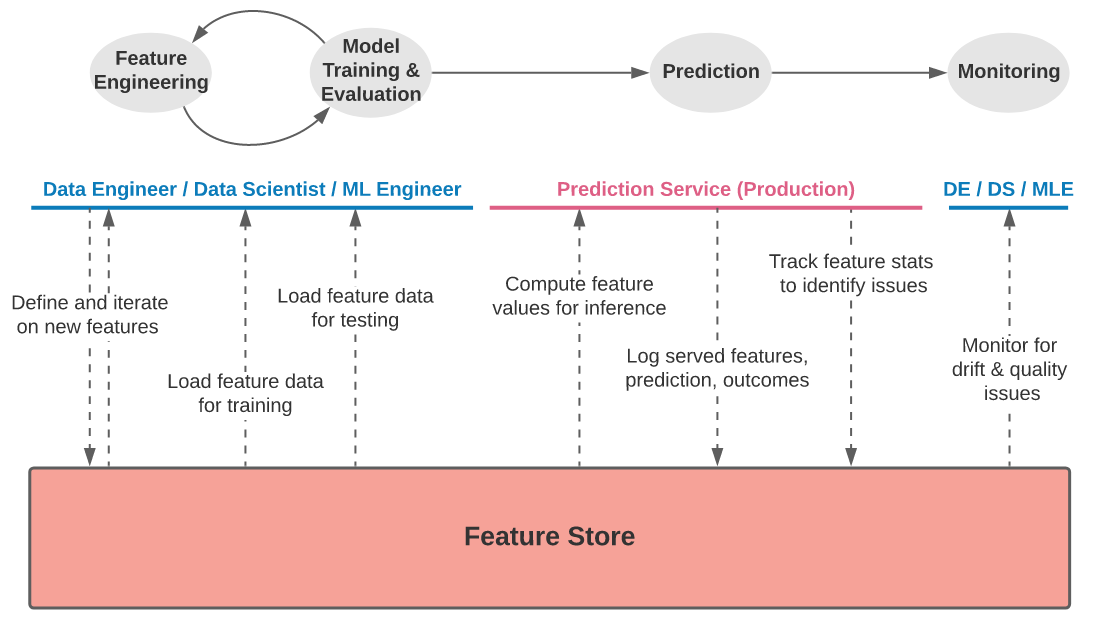
\includegraphics[width=\textwidth-10pt]{book-text/feature-store.png}
\end{figure}

Designing a feature store involves designing pipelines that define and \emph{transform the features into that store}–coordinated via things like Airflow, Luigi, Argo, etc.–and often look similar to the type of data pipelines used in building our collector. One additional complication that the feature store needs to concern itself with is a speed layer. We mentioned before that for the collector, we can think of batch data processing and a more rapid speed layer for intermediary updates, but for the feature store this is even more important. The feature store may also need a \emph{streaming layer}. The streaming layer is something that operates on continuous streams of data, and can perform data transformations on those; it then writes the appropriate output to the online feature store in real time. The reason this adds complexity is because data transformations on streaming data are a very different set of challenges, and often require different algorithmic strategies. Some technologies that help here are Spark Streaming or Kinesis. You'll also need to configure system to properly handle the data stream; the most common of which is Kafka.

A feature store also needs a \emph{storage layer}; a large variety of different approaches exist here, but it's very common to use a NoSql database especially in the online feature store. This is because of faster retrieval and the nature of the data storage. Feature stores for recommendation systems tend to be very key-based, i.e. 'get the features for this user', or 'get the features for this item', which lend themselves well to key-value stores. Some example technologies here are DynamoDB, Redis, and Cassandra. The storage layer for offline feature store may simply be a Sql style database to reduce complexity, but instead you'll pay a tax of a delta between offline-and-online. This delta, and others like it are call [training-serving skew]\url{https://developers.google.com/machine-learning/guides/rules-of-ml#:~:text=Training%2Dserving%20skew%20is%20a,train%20and%20when%20you%20serve.}).

A unique but essential aspect of feature stores is the \emph{registry}. A registry is incredibly useful for a feature store because it coordinates what features exist, and some information on how they're defined. A more sophisticated instance of a registry also includes input and output schemas with typing, and distributional expectations. These things are contracts that the data pipelines must adhere to and satisfy to avoid populating your feature store with garbage data. Additionally the registry's definitions allow parallel Data Scientists and ML Engineers to develop new features, use each others features, and generally understand the assumptions of features their models may utilize. One important advantage of these registry is that they incentivize alignment between teams and developers–in particular, if you decide you care about 'country' for your user, and you see that there is a feature 'country' in the registry, you're more likely to just use that (or ask the developer who's assigned to this feature in the registry) than make a new one from scratch. Practically, there are hundreds of small decisions and assumptions data scientists make when defining features for their models, this removes some of that load be relying on the existing resources.

Finally, we need to talk about \emph{serving} these features. Backed by the appropriately performant storage layer, we need to serve via API request the feature vectors necessary. The API can serve back the entire set of features for the key, or allow for more specification. Often the responses are JSON serialized for fast data transfer. It's important that the features be served are the \emph{most up to date set of features}, and latency here is expected to be <100ms for more serious industrial applications. One important caveat here is that for offline training, these feature stores need to accommodate \emph{time-travel}. Because our goal during training is to give the model the appropriate data to learn in the \emph{most generalizable way}, when training our model it's crucial to not give it access to features out of time. This is called \emph{data-leakage} and can cause massive divergence in performance between training and prod. The feature store for offline training thus must have knowledge of the features through time, so that during training, a time index may be provided to get the features as they were then. These \lstinline{as_of} keys can be tied to the historical training data as we 'replay' history of what the user-item interactions looked like.

With these pieces in place–and the important monitoring this system needs–you'll be able to serve offline and online features to your models. Later we will see model architectures that make use of them.

\paragraph{Data leakage}

Data leakage in machine learning is broken up into \emph{feature leakage} and \emph{training example leakage}. For recommendation systems, data leakage has the additional challenge of temporal leakage or non-stationarity leakage. The real danger is that in recommendation systems, we see the same observational unit, a user, over and over, and observe a datum each time we see them. When we see them, other aspects of the system may have changed, and in reality we want to use features in our model that are the most up-to-date as of that observation. Both in features and training examples, to avoid leakage we need to always be thinking of the timeline of our system. This is why data preparation for recommendation systems is inherently time-dependent. We will see later that our accuracy metrics will need to explicitly consider train-test splitting with respect to this time axis, and then further grouped by the user. This also means that training recommendation systems often requires more resources than many other task types.

\chapter{Serving models and architectures}
\label{ch:serving-and-architecture}

\section{Architectures by recommendation structure}

We have returned several times to the concept of Collector, Ranker, Server, and we've seen that those may be considered via two paradigms: the online and the offline modes. Further, we've seen how many of the components in the last chapter on data processing satisfy some of the core requirements of these functions.

In designing large systems like these, there are a number of architectural considerations. Now we'd like to demonstrate how these concepts adapt based on the type of recommendation system you are building. For this purpose we compare a mostly standard item-to-user recommendation system, a query-based recommendation system, contextual recommendations, and sequence-based recommendations.

\subsection{Item-to-user recommendations}

First up is the system we've been discussing thus far! As proposed in [4 System Design for Recommendation Systems](https://www.notion.so/4-System-Design-for-Recommendation-Systems-adfc961643194fa295c799ac2dfc300e), we build the collector offline to ingest and process our recommendations. We utilize representations to encode relationships between items, users, or user-item pairs. The online collector takes the request, usually in the form of a user-id, and finds a neighborhood of items in this representation space to pass along to the ranker. Those items are filtered when appropriate and sent for scoring. The offline ranker trains the relevant features for scoring and ranking, training on the historical data. The online ranker uses this model and potentially the necessary features for inference. In the case of recommendation systems this inference is the scores associated to each item in the set of potential recs. We usually sort by this score. Finally, we integrate a final round of ordering based on some business logic. This last step is part of the serving where we impose things like test-criteria or recommendation diversity requirements.

\begin{figure}[h!]
    \caption{This image by Karl Higley and Even Oldridge is an excellent overview of the architecture we've just described. (used with permission)}
    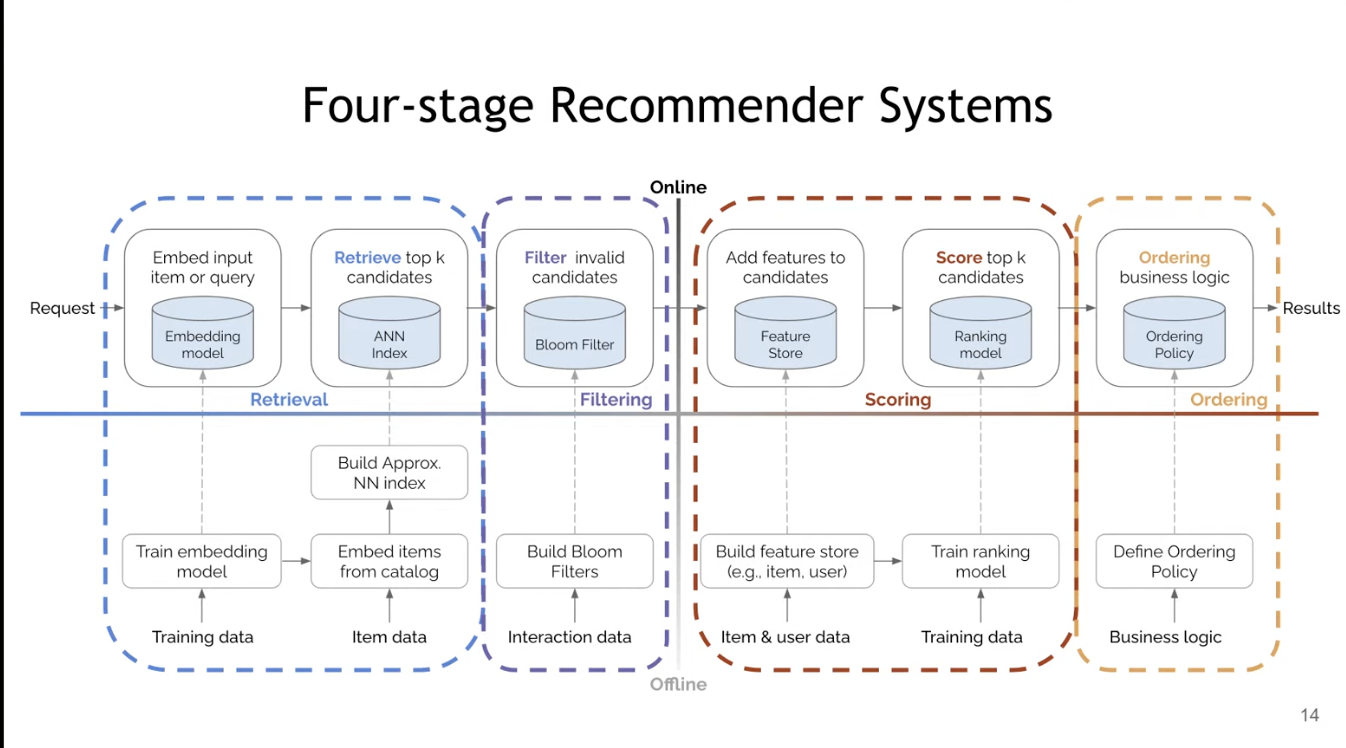
\includegraphics[width=\textwidth-10pt]{book-text/four-stage-diagram.png}
\end{figure}

\subsection{Query-based recommendations}

Next we want to include a query to start off our process. The most obvious example of a query is a text query like in text-based search engines. However, queries may be more general! For example you may wish to allow search-by-image, or search-by-tag. While these systems are quite similar in overall structure to the above, let's discover how to modify them to fit our use-case.

Immediately, we wish to integrate something more into the first step of the request. Note that we don't want to throw out the user-item matching components of this system\textemdash even though the user is performing a search, there's utility in personalizing the recommendations based on their taste. So now we need to utilize the query in addition; later we will discuss various technical strategies, but a simple summary for now is to also train an embedding for the query! Note that the query is like and item, but sufficiently different. Some strategies might include similarity between the query and items, or co-occurrence of the query and items. Either way, we now have a query representation and user-representation, and we want to utilize both for our recommendation. One simple strategy here is to use the query representation for retrieval, but during the scoring, score via both query-item and user-item, combining them via a multi-objective loss. Another strategy is to use the user for retrieval, and then the query for filtering. 

\subsection{Context-based recommendations}

A context is actually quite similar to a query, but tends to be more obviously feature based. Context is usually the term use to represent some exogenous features to the system, that may have an effect on the system, i.e. auxiliary information such as time, weather, location, and more. The ways in which it is similar to query-based recommendation are that it's an additional signal that the system needs to consider during recommendation, but more often than not: query should dominate the signal for recommendation, whereas context should not. 

Let's take a simple example: when ordering food. A query for a food-delivery recommendation system would look like 'Mexican food'; an extremely important signal from the user of how the recs should look. A context for a food-delivery recommendation system would look like 'it's almost lunch time'; a useful signal, but either equally weighted with user-personalization or lesser. It's hard to put hard and fast rules on this weighting, so usually we don't, and just learn parameters via experimentation.

How they fit into the architecture is very similar to queries, but via these features. Learn a representation between context features and items, and add that affinity into the rest of the pipeline. Again you can make use of this early in the retrieval, later in the ranking, or even during the ordering step. 

\subsection{Sequence-based recommendations}

Sequence based recommendations builds on context-based recommendations, but with a specific type of context. Sequential recommendations are the concept that the lagging items the user has been exposed to should have a significant influence on the recommendations. A common example here is a music streaming service, where the last few songs that have been played can significantly help inform what the user might want to hear next. To ensure this 'auto-regressive' set of features has an influence on recommendations, we can treat each item in the sequence as a weighted context for the recommendation.

Usually, the item-item representation similarities are weighted to provide a collection of recommendations and various strategies are used for combining these. In this case, we normally expect the user to be of high importance in the recommendations but the sequence is also of high importance. One simple model is to think of the sequence of items like a sequence of tokens, and form a single embedding for that sequence\textemdash like in NLP applications. This embedding can be used as the context in a context-based recommendation architecture.

\subsection{Aside: Why bother with extra features}

Sometimes it is useful to step back and ask if a new technology is actually worth caring about. So far in this section we've introduce four new paradigms for how to think about a recommender problem. That may seem surprising and potentially even unnecessary. 

One of the core reasons that things like context and query based recommendations become relevant is to deal with some of the issues mentioned before around sparsity and cold-starting. Sparsity makes things that aren't cold seem cold via the learner's under-exposure to them, but true cold starting also exists due to new items being added to catalogs all the time in most applications. We will address cold-starting in detail, but for now, suffice to say that one strategy for warm starting is to use other features which *are* available even in this regime.

In applications of machine learning that are explicitly feature based, we rarely battle the cold-start problem to such a degree, because at inference time we're confident that the model parameters useful for prediction are well aligned with those features that are available. In this way, feature-included recommendation systems are bootstrapping from a potentially weaker learner, that has more guaranteed performance via always available features. 

The second analogy that the previous architectures are reflecting is that of boosting. Boosted models operate via the observation that ensembles of weaker learners can reach better performance. Here we are asking for some additional features to help these networks ensemble with weak learners, to boost their performance. 

\section{Encoder architectures \& cold starting}

The previous problem framings of different types of recommendation problems points out four model architectures, each fitting into our general framework of collector, ranker, server; now let's discuss in a bit more detail how model architecture can become intertwined with serving architecture. In particular, we also wish to discuss feature encoders. 

The key opportunity from encoder-augmented systems is that for users, items, or contexts without much data, we can still form embeddings on the fly. Recall from before that our embeddings made the rest of our system possible, but cold-starting recommendations was a huge problem.

The \emph{two-towers architecture}\textemdash \emph{or dual encoder networks}\textemdash introduced in [Yi et. al.]\url{https://storage.googleapis.com/pub-tools-public-publication-data/pdf/6c8a86c981a62b0126a11896b7f6ae0dae4c3566.pdf}, is an explicit model architecture aimed at prioritizing features of both the user and items, when building a scoring model for a recommendation system. Our previous discussion of matrix factorization described it as a collaborative filter, focused on utilizing implicit similarity via interaction to provide our affinities. From last section, it is now obvious to you that additional features matter. While adding these \emph{side-car} features into a matrix factorization paradigm is possible and has shown to be successful, c.f. [[CF for Implicit Feedback]\url{http://yifanhu.net/PUB/cf.pdf}, [Factorization Machines]\url{https://www.csie.ntu.edu.tw/~b97053/paper/Rendle2010FM.pdf}, [SVDFeature]\url{http://wnzhang.net/papers/svdfeature-jmlr.pdf}, in this model we will take a more direct approach. 

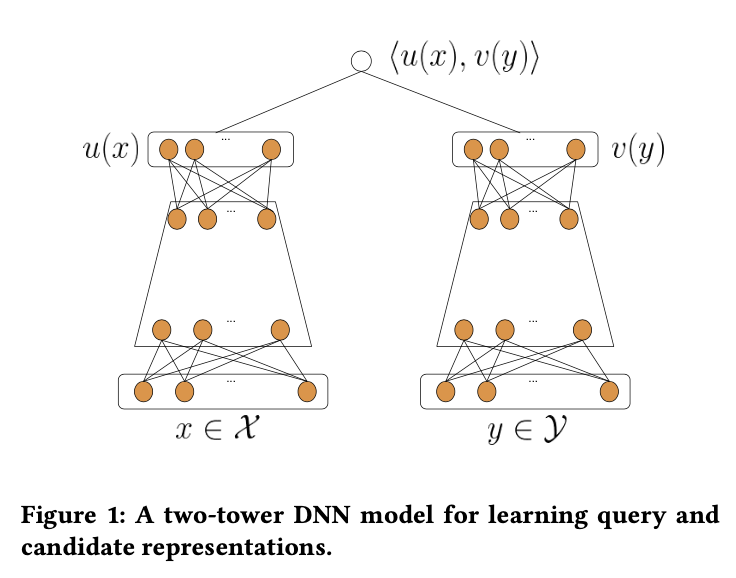
\includegraphics[width=\textwidth-10pt]{book-text/two-towers-architecture-diagram.png}

In this architecture, we take the left tower to be responsible for items, and the right tower to be responsible for user\textemdash and when appropriate\textemdash context. These two tower architectures are inspired from the NLP literature and in particular the [Learning Text Similarity](https://aclanthology.org/W16-1617.pdf) work. 

Let's work through in detail how this model architecture is applied to recommending videos on YouTube. Note that this follows the paper introducing this architecture. Training labels will be given by clicks, but with an additional regression feature $r_i\in [0,1]$ where the minimum value corresponds to click but trivial watch-time, and the maximum of the range corresponds to a full-watch. 

As mentioned above, this model architecture will explicitly include features from both user and items. The video features will consist of categorical and continuous features, like \lstinline{VideoId}, \lstinline{ChannelId}, \lstinline{VideoTopic}, and so on. An embedding layer is used for many of the categorical features to move to dense representations. The user features are things like watch histories via bag of words, and standard user features.

This model structure combines many of the ideas we've seen before, but has relevant takeaways for our system architecture. First, is the idea of sequential training. Each 'temporal batch' of samples, should be trained in sequence to ensure that model drift is shown to the model. Next, we see an important idea for the productionizing of these kinds of models:  encoders.

In these models, we have feature encoders as the early layers in both towers, and when we move to inference, we will still need these encoders. When performing the online recommendations, we will be given \lstinline{user_id} and \lstinline{video_id}, and first need to collect their features. As discussed before, the Feature Store will be useful in getting these raw features, but we need to also encode into the dense representations necessary for inference. This is something that can be stored in the feature store for known entities, but for unknown entities we will need to do the feature embedding at inference time.

Encoding layers serve as a simple model for mapping a collection of features to a dense representation. When fitting encoding layers as the first step in a neural network, the common strategy is to take the first $k$ layers and re-use them as an encoder model. More specifically, if $\mathcal{L}^i, 0\leq i\leq k$ are the layers responsible for feature encoding, call $Emb(\hat{V})=\mathcal{L}^k(\mathcal{L}^{k-1}(\ldots\mathcal{L}^0(\hat{V})))$ the function which maps a feature vector $\hat{V}$, to it's dense representation.

In our previous system architecture, we would include this encoder as part of the fast layer, after receiving features from the feature store. It's also important to note that we would still want to utilize vector search; these feature embedding layers are used upstream of the vector search and nearest neighbor searches.

\section{Deployment}

Like many applications of Machine Learning, the final output of a recommendation systems is itself a small program that runs continuously and exposes an API to interact with it. In much of what we've already done this chapter, we've seen the pieces embedded in that system, but now we should discuss the components closer to the user. 

In our relatively general architecture, the server is responsible for handing over the recommendations, after all the work that comes before and it should adhere to a preset schema. But what does this deployment look like?

\subsection{Models as APIs}

Let's discuss two systems architectures that might be appropriate for serving your models in production: micro-service and monolith.

In web applications this dichotomy is well covered from many perspective and special use-cases. As ML engineers, Data Scientists, and potentially Data Platform engineers, it's not necessary to dig deep into this area, but it's essential to know the basics. Simply: \emph{micro-service architectures} state that each component of the pipeline should be it's own small program with clear API and output schema, composing these API calls allow for flexible and predictable pipelines. In contrast, \emph{monolithic architectures} suggest that one application should contain all the necessary logic and components for model predictions, keeping the application self-contained means less interfaces that need to be kept aligned and less rabbit holes to hunt in when some location in your pipeline is being starved.

Whatever you choose as your strategy, you'll need to make a few decisions:

\begin{itemize}
\item How large is the necessary application? If your application will need fast access to large dataset at inference time, you'll need to think carefully about memory requirements.
\item What access does your application need? We've previously discussed making use of things like Bloom filters, and Feature stores; these resources may be tightly coupled to your application\textemdash by building them in memory in the application\textemdash or they might be an API call away. Make sure your deployment accounts for these relationships.
\item Should your model be deployed to a single node or a cluster? For some types of model, even at the inference step we wish to utilize distributed computing. This will require additional configuration to allow for fast parallelization.
\item How much replication do you need? \emph{Horizontal scaling} allows you to have multiple copies of the same service running simultaneously to reduce the demand on any particular instance. This is important for ensuring availability and performance. As we horizontally scale, each service can operate independently and there are different strategies for coordinating these services and an API request. Each replica is usually it's own containerized application and things like CoreOS and Kubernetes are used to manage these. The requests themselves must also be balanced to the different replicas via something like NGINX.
\item What are the relevant API's exposed? Each application in the stack should have a clear set of exposed schemas, and an explicit communication about what types of other applications may call to them.
\end{itemize}

\paragraph{Spinning up a model service}

So what can you use to actually get your model into an application? One of a variety of frameworks for application development are useful; some of the most popular in Python are Flask, FastAPI, and Django. Each have different advantages, but we'll choose to discuss here FastAPI. 

FastAPI is a targeted framework for API applications, making it especially well fit for serving ML models. It calls itself an ASGI (Asynchronous Server Gateway Interface) framework; and it's specificity grants a ton of simplicity. 

Let's take a simple example of turning a fit torch model into a service with the FastAPI framework. First, let's utilize an artifact store to pull down our fit model; here we are using Weights and Biases artifact store:


\begin{lstlisting}[language=python]
import wandb, torch
run = wandb.init(project=Prod_model, job_type="inference")

model_dir = run.use_artifact(
		'bryan-wandb/recsys-torch/model:latest', 
		type='model'
).download()

model = torch.load(model_dir)
model.eval(user_id)
\end{lstlisting}

This looks just like your notebook workflow, so let's see how easy it is to integrate this with FastAPI:

\begin{lstlisting}[language=python]
from fastapi import FastAPI # FastAPI code

import wandb, torch

app = FastAPI() # FastAPI code

run = wandb.init(project=Prod_model, job_type="inference")

model_dir = run.use_artifact(
	'bryan-wandb/recsys-torch/model:latest', 
	type='model'
).download()

model = torch.load(model_dir)

@app.get("/recommendations/{user_id}") # FastAPI code
def make_recs_for_user(user_id: int): # FastAPI code
		endpoint_name = 'make_recs_for_user_v0'
		logger.info(
			"{'type': 'recommendation_request'," 
			f"'arguments': {'user_id': {user_id}}," 
			f"'response': {None}},",
			f"'endpoint_name': {endpoint_name}"
		)
		recommendation = model.eval(user_id)
		logger.log(
			"{'type': 'model_inference'," 
			f"'arguments': {'user_id': {user_id}}," 
			f"'response': {recommendation}},"
			f"'endpoint_name': {endpoint_name}"
		)
    return { # FastAPI code
			"user_id": user_id, 
			"endpoint_name": endpoint_name, 
			"recommendation": recommendation
		}
\end{lstlisting}

I cannot stress enough that via only we now have a model-as-a-service in five additional lines of code. We will see more discussion about logging later to help you improve observability in all of your applications, but here I included some very simple examples of logging. 

\section{Alerting and Monitoring}

Alerting and monitoring take a lot of their inspiration from the DevOps world for software engineering. Some high level principles which will guide our thinking are:

\begin{itemize}
\item clear defined schemas and priors
\item observability
\end{itemize}

\subsection{Schemas and Priors}

When designing software systems, you almost always have expectations of how the components fit together. Much like in writing code you anticipate the input and output to functions, in software systems you anticipate these at each interface. Not only for micro-service architectures is this relevant; even in a monolith architecture components of the system need to work together and often will have boundaries between their defining responsibilities. 

Let's make this more concrete via an example: you've built a user-item latent space, a feature store for user features, a bloom filter for client avoids, and an experiment index which defines which of two models should be used for scoring. First let's examine the latent space: when provided a \lstinline{user_id} we need to look up its representation, and we have some assumptions already:

\begin{itemize}
\item \lstinline{user_id} provided will be of the correct type
\item \lstinline{user_id} will have a representation in our space
\item The representation returned will be of the correct type and \lstinline{shape}
\item The component values of the representation vector will be in the appropriate domain. \emph{(Note: the support of representations in your latent space may vary day-to-day)}
\end{itemize}

From here, we need look up the $k$ Approximate Nearest Neighbors, which incurs more assumptions:

\begin{itemize}
\item There are $\geq k$ vectors in our latent space
\item Those vectors adhere to the expected distributional behavior of the latent space
\end{itemize}

While these seem relatively straightforward application of unit-tests, canonizing these assumptions is important. Take the last assumption in both of the two services: how can you know the appropriate domain for the representation vectors? As part of your training procedure, you'll need to calculate this, then store it for access during the inference pipeline. 

In the second case, when finding nearest neighbors in high dimensional spaces, there are well discussed difficulties in distributional uniformity, but this can mean particularly poor performance for recommendations. In practice, the authors have observed a spiky nature to the distribution of $k$-NN in latent spaces, leading to difficult challenges downstream in ensuring diversity of recommendations. These distributions can be estimated as priors and simple checks like KL-divergence can be used online. 

In both cases, collecting the output of this information and logging it can provide a rich history of what is going on with your system; this can shorten debugging loops later on if model performance is low in production.

Returning to the possibility of \lstinline{user_id} lacking a representation in our space: this is precisely the cold-start problem! In that case we need to transition over to a different prediction pipeline: perhaps user-feature-based, explore-exploit, or even hard-coded recommendations. In this setting, we need understand next steps when a schema condition is not met and gracefully move forward. 

\paragraph{Integration tests}

Let's consider one higher-level challenge that might emerge in a system like this at the level of integration. Some refer to these issues as \emph{entanglement.}

You've found through experimentation that you should find $k=20$ approximate nearest neighbors in the item-space for a user to get good recommendations. You make a call to your representation space, get your 20 items, and pass them onto the filtering step. However, this user is quite picky; they have previously made many restrictions on their account about what kind of recommendations they allow: no shoes, no dresses, no jeans, no hats, no handbags \textemdash what's a struggling RecSys to do! 

Naively, if you take the 20 neighbors, and pass them into the bloom, you're likely to be left with nothing! There are two ways to approach this challenge:

\begin{itemize}
\item allow for a call-back from the filter step to the retrieval
\item build a user-distribution and store that for access during retrieval
\end{itemize}

In the first of these, you give access to your filter step to call the retrieval step with a larger $k$ until the requirements are satisfied after the bloom. Of course, this incurs significant slow-down as it requires multiple passes and ever growing queries with redundancy! While this approach is simple, it requires building defensively and knowing ahead of time what may go wrong.

In the second of these, during training, you can sample from the user space to build estimates of the appropriate $k$ for varying numbers of avoids by user. Then giving access to a lookup of total avoids-by-user to the collector can help defend against this behavior.

\subsection{Observability}

There are quite a number of tools in the software engineering to assist with observability, understanding the why's of what's going on in the software stack. Because the systems we are building become quite distributed, the interfaces become critical monitoring points, but the paths also become complex.

Common terms in this area are \emph{spans} and \emph{traces,} which refer to two dimensions of a call stack. Given some collection of connected services, like in our above examples, an individual inference request will pass through some or all of those services in a sequence. The sequence of service requests is the trace. The, potentially parallel, time-delays of each of these services, is the span. 

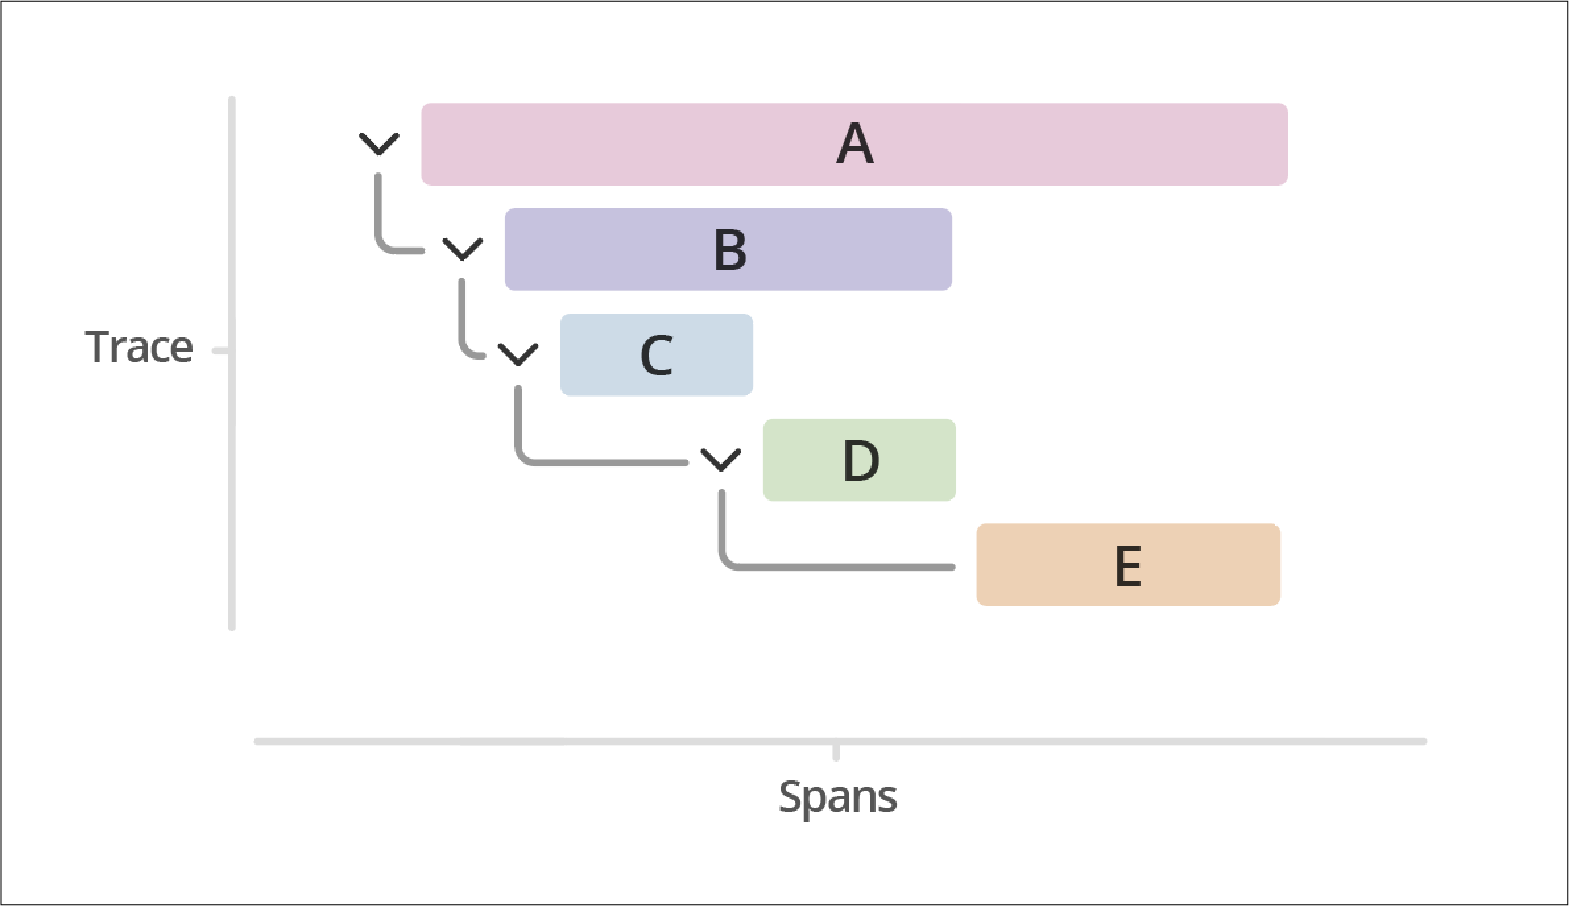
\includegraphics[width=\textwidth-10pt]{book-text/trace-spans.png}

The graphical representation of spans usually demonstrates how the time for one service to respond is comprised of several other delays from other calls. 

Observability is being able to see traces, spans, and logs in conjunction to appropriately diagnose the behavior of your system. In our example above where we utilize a call-back from the filter step to get more neighbors from the collector, we might see a slow response and wonder "what has happened?". By viewing the spans and traces, we'd be able to see that the first call to the collector was as expected, then the filter step made a call to the collector, then another call to the collector, and so on, which built up a huge span for the filter step. Combining that view with logging would help us rapidly diagnose what might be happening.

\paragraph{Time-outs}

In the above example, we had a long process that could lead to very bad user experience. In most cases, we impose hard restrictions on how bad we let things get; these are called time-outs. 

Usually we have an upper bound on how long we're willing to wait for our inference response, and so implementing time-outs aligns our system with these restrictions. It's important in these cases to have a \emph{fall-back.} In the setting of recommendation systems, a fall-back is usually comprised of things like the MPIM prepared such that it incurs minimal additional delay. 

\section{Evaluation in Prod}

If the previous section was understanding what's coming into your model in production, this might be summarized as what's coming out of your model in production. At a high level, evaluation in Prod can be thought of as extending all your model validation techniques to the inference time. In particular, *what the model actually is doing!*

On one hand we already have tools to do this evaluation \textemdash you can use the same methods used for evaluating performance as in training, but now on real observations streaming in. However, this is not as obvious as we might first guess.

\paragraph{Slow feedback}

Recommendation systems fundamentally are trying to lead to item selection, and in many cases, purchases. But if we step back and think more holistically about how recommendation systems integrate into businesses, it's to drive revenue. If you're an e-commerce shop, item selection and revenue may seem easily associated: a purchase leads to revenue, so good item recommendation leads to revenue. However, what about returns? Or even a harder question: are these revenue incremental? One challenge with recommendation systems, is there may sometimes be a very difficult to draw causal arrow between any metric used to measure the performance of your models to the business-oriented key performance indicators.

We call this slow feedback because sometime the loop to get from a recommendation, to a meaningful metric, and back to the recommender can take weeks or even longer. This is especially challenging when you want to run experiments to understand if a new model should be rolled out. The length of the test may need to stretch quite a bit more to get meaningful results. 

Usually a proxy metric is aligned on that the data scientists believe is a good estimator for the KPI, and that proxy metric is measured live. There are a huge variety of challenges with this approach, but it often suffices and provides motivation for more testing. 

\paragraph{Model metrics}

So what are the key metrics to track for your model in prod? Given that we're looking at recommendation systems at inference time, we should seek to understand:

\begin{itemize}
\item distribution of recommendation across categorical features
\item distribution of affinity scores
\item number of candidates
\item distribution of other ranking scores
\end{itemize}

As we discussed before, during the training process, we should be calculating broadly what the ranges of our similarity scores are in our latent space. While we can look at high level estimations, or finer ones, we can use these distributions to get warning signals something might be strange. Simply comparing the output of our model during inference, or over a set of inference requests, to these pre-compute distributions can be extremely helpful.

Comparing distributions can be a long topic, but one standard approach is \emph{KL-Divergence} between the observed distribution, and the expected distribution from training. By computing KL-Divergence between these, we can understand how 'surprising' the model's predictions are on a given day. 

What we'd really like is to understand the ROC of your model predictions with respect to one of your conversion types. However, this involves yet another integration to tie back to logging. Since your model API only produces the recommendation, you'll still need to tie into logging from the web application to understand outcomes! To tie back in outcomes one must join the model predictions with the logging output to get the evaluation labels, which can be done via log parsing technologies (like ELK or Prometheus). We'll see more of this in the next chapter. 

\section{Continuous training and deployment}

It may feel like we're done with this story since we have models tracked and production monitoring in place, but rarely are we satisfied with set-it-and-forget-it of model development. One important characteristic of ML products, is how models frequently need to be updated to even be useful. Above we discussed model metrics, and how sometimes performance in production might look different than what we had come to expect from the trained models' performance. This can even be further exacerbated by \emph{model drift.}

Model drift is the notion that the same model may exhibit different prediction behavior over time, merely due to changes in the data generating process. A very simple example is a time-series forecasting model. When you build a time-series forecast model, the specially unique property that is essential for good performance is \emph{auto-regression,} that is to say that the value of the function covaries with previous values of the function. We wont go into detail on time-series forecasting, but suffice to say: the best hope you have of making a good forecast is to use up-to-date data! If you wanted to forecast stock prices, you'd always want to use the most recent prices as part of your predictions. This simple example demonstrates how models may drift; a model that did well two weeks ago, needs to be retrained with recent data to be expected to continue to perform well.

One criticism of a model that drifts is "that's the smoking gun of an overfit model", but in reality these models require a certain amount of over-parameterization to have useful models. In the context of recommendation systems, we've already seen things like the Matthew Effect can have disastrous effects on the expected performance of a recommender model. If we don't consider thinks like new items in our recommender, we are doomed to fail. Models can drift for a variety of reasons, often coming down to exogenous factors in the generating process that may not be captured by the model. 

One approach to dealing with and predicting stale models, is to simulate these scenarios during training. If your expectation is that the model goes stale mostly due to the distribution changing over time, you can employ sequential cross-validation \textemdash  i.e. train on a contiguous period and test on a subsequent period \textemdash but with a specified block of time delay. For example, if you think your model performance is going to decrease after two week due to being trained on out-of-date observations, then during training you can purposely build your evaluation to incorporate a two-week delay before measuring performance. This is called \emph{two-phase prediction comparison} and by comparing the performances you can estimate drift magnitudes to keep an eye out in prod. 

There are a wealth of statistical approaches to reigning in these differences; in lieu of a deep dive into variational modeling for variability and reliability for your predictions, we'll instead discuss continuous training and deployment and open this peanut with a sledge hammer.

\subsection{Deployment topologies}

Let's consider a few different structures for how you want to deploy models to not only keep your models well in tune, but to accommodate iteration, experimentation, and optimization.

\paragraph{Ensembles}

Ensembles are a type of model structure in which multiple models are built, and the predictions from those models are pooled together in one of a variety of ways. While this notion of an ensemble is usually packaged into the model called for inference, you can actually generalize the idea to your deployment topology. Let's take an example that builds on our previous discussion of prediction priors. If we have a collection of models with comparable performance on a task, we can deploy them in ensemble weighted by their deviation from the prior distributions of prediction that we've set before. This way, instead of having a simple yes/no filter on the output of your model's range, you can more smoothly transition potentially problematic predictions into more expected ones. 

Another benefit of treating the ensemble as a deployment topology instead of only a model architecture, is that you can 'hot-swap' components of an ensemble as you make improvements in specific sub-domains of your observation feature space. Take for example an LTV model comprised of three components, one that predicts well for new clients, another for activated clients, and a third for super-users. You may find that pooling via a voting mechanism on average performs the best, so you decide to implement a bagging approach. This works well, but later you find a better model for the new clients. By using deployment topology for your ensemble you can swap in the new model for the new clients, and start comparing performance in your ensemble in prod. This brings us to the next strategy, model comparison.

\paragraph{Shadowing}

Deploying two models, even for the same task, can be enormously informative. We call this shadowing in the case where one model is "live" and the other is secretly also receiving all the requests and doing inference, and logging the results of course. By shadowing traffic to the other model, you get the best expectations possible about how the model behaves before making your model live. This is especially useful when wanting to ensure that the prediction ranges align with expectation. 

In software engineering and devOps, there's a notion of \emph{staging} for software. It's a hotly contested question of "how much of the real infra should staging see", but shadowing is the staging of ML models. You can basically build a parallel pipeline for your entire infrastructure to connect for shadow models, or you can just put them both in the line of fire and have the request sent to both, but only use one response. Shadowing is also crucial for implementing experimentation.

\paragraph{Experimentation}

As good data scientists, we know that without a proper experimental framework, it's risky to advertise much about the performance of a feature or in this case model. Experimentation can be handled with shadowing by having a controller layer that is taking the incoming requests and orchestrating which of the deployed models to curry the response along from. A simple A/B experimentation framework might ask for a randomization at every request, where-as something like a multi-armed bandit will require the controller layer to have notions of the reward function.

Experimentation is a deep topic which we don't have the knowledge or space to do adequate justice, but it's useful to know that this is where experimentation can fit into the larger deployment pipeline.

\paragraph{Aside: Model Cascades}

A really nice extension of several of the ideas is one of \emph{Model Cascading.} The simplified idea of a model cascade is that we use model confidence to create a conditional ensemble. In particular, given an inference request the model provides a prediction with a confidence estimate; when the model confidence is high that prediction is returned, but if the confidence is below some threshold, a downstream model is called and the ensemble is started. There's no reason to stop at two, for any number of models that in training show improved performance in ensemble, this method can be used to iteratively expand the number of ensemble layers. 

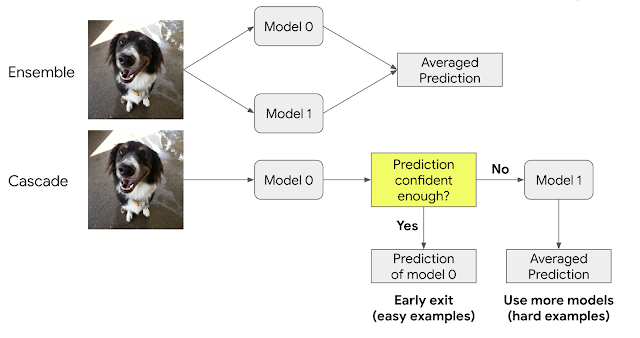
\includegraphics[width=\textwidth-10pt]{book-text/model-cascades.png}

A few advantages of this approach are:

\begin{itemize}
\item better expected performance overall; ensembles usually increase performance
\item ensemble performance with lower average computation time
\item especially better performance in out-of-sample scenarios
\end{itemize}

This method scales to larger pools of models and while it may incur significant training efforts, finding the right ordering of the models can have significant effects on model accuracy and latency.

\chapter{The evaluation flywheel}
\label{ch:serving-and-architecture}

By now it's likely obvious that a production ML model is far from a static object. Production ML systems of any kind are subject to as many deployment concerns as a traditional software stack, in addition to the added challenge of dataset shift and new users/items. In this section we want to look closely at the feedback loops introduced and understand how the components fit together to continuously improve our system–even with little input from a data scientist or ML Engineer.

\section{Daily warm-starts}

As we've now discussed several times, there need be a connection between the continuous output of our model and retraining. The first simplest example of this is daily warm-starts, which essentially asks us to utilize the new data seen each day in our system.

As might already be obvious, some of the recommendation models that show great success are quite large. Retraining some of them can be a massive undertaking, and simply 'rerunning everything' each day is often infeasible. So what can be done? 

Let's ground this conversation in the user-user collaborative filtering example that we've been sketching out; we have seen that the first step was to build an embedding via our similarity definition. Let's recall:

\begin{equation}
\mathrm{USim}_{A,B}=\frac{\sum_{x\in \mathcal{R}_{A,B}}(r_{A,x}-\bar{r}_A)(r_{B,x}-\bar{r}_B)}{\sqrt{\sum_{x\in \mathcal{R}_{A,B}}(r_{A,x}-\bar{r}_A)^2} \sqrt{\sum_{x\in \mathcal{R}_{A,B}}(r_{B,x}-\bar{r}_B)^2}}
\end{equation}

here we remember that the similarity between two users is dependent on the shared ratings, and by each user's average rating. 

On a given day, let's consider $\tilde{X}=\left\lbrace \tilde{x}\mid x\textrm{ was rated since yesterday by some user }\right\rbrace$, then we need to update our user similarities, but ideally we'd leave everything else the same. To update the above, we see that all $\tilde{x}$ rated by two users, $A$ and $B$, will contribute changes. One also might notice that the $\bar{r}_A$ and $\bar{r}_B$ would need to change, but we could probably skip these updates in many cases where the number of ratings by those users was large. All in all, this means for each $\tilde{x}$ we should look up which users previously rated $x$ and update the user similarity between them and the new rater. 

This is a bit ad\-hoc, but for many methods you can utilize these tricks to reduce a full retraining. This would avoid a full batch retraining, via a fast-layer. There are other approaches to this like building a separate model that can approximate recs for low-signal items. This can be done via feature models, and can significantly reduce the complexity of these quick re-trainings.

\subsection{Lambda architecture and orchestration}

On the more extreme end of the spectrum of these strategies is the lambda architecture; as discussed during our data hydration discussions, the lambda architecture seeks to have a much more frequent pipeline for adding new data into the system. The speed layer is responsible for working on small batches to perform the data transformations, and model fitting to combine with the core model. As we discussed before, there's a bunch of other aspects of the pipeline that should also be updated during these fast layers, like the nearest neighbors graph, the feature store, and the filters. 

Different components of the pipeline can require different investments to keep updated, so it's an important consideration what kinds of schedules they are on. You might be starting to notice that keeping all of these things in sync can be a bit challenging–if you have model training, model updating, feature store updates, redeployment, and new items/users all coming in on potentially different schedules, there can be a *lot* of coordination necessary. This is where an \emph{orchestration tool} can become relevant. There are a variety of approaches but a few useful technologies here are GoCD, MetaFlow, and KubeFlow; the latter being more oriented at Kubernetes infrastructures. Another pipeline orchestration tool that can handle both batch and streaming pipelines is Apache Beam.

Generally, for ML deployment pipelines we need to have a reliable core pipeline, and the ability to keep things up-to-date as more data pours in. Orchestration systems usually define the topology of the systems, the relevant infrastructure configurations, the mapping of the code artifacts needing to be run, and the CRON schedules when all as code itself. Code-as-infrastructure is a popular paradigm which captures these goals as a mantra, so that even all of this configuration itself is reproducible and automatable. 

In all of the above, there's a heavy overlap with containerization and *how* these things may be deployed. Unfortunately most of this discussion is beyond the scope of this book, but a simple overview is that containerized deployment with something like Docker is extremely helpful for ML Services and managing those deployments with various container management systems, like Kubernetes, is also popular.

\section{Logging}

Logging has come up several times already, in model monitoring and our schema assumptions sections we saw that logging was very important for insuring that our system was behaving as expected. Let's discuss some best practices for logging, and how they fit into our plans.

When we discussed traces and spans earlier, we were able to get a snapshot of the entire call-stack of the services involved in responding to a request. This concept of linking together the services to see the larger picture is incredibly useful, and when it comes to logging gives us a hint as to how we should be orienting our thinking. Returning to our favorite RecSys architecture we have:

\begin{itemize}
\item Collector receiving the request and looking up the embedding relevant to the user
\item Computing ANN on items for that vector
\item Applying filters via blooms to eliminate potential bad recs
\item Feature augmentation to the candidate items and user via the feature stores
\item Scoring of candidates via the ranking model, and potential confidence estimation
\item Ordering and application of business logic or experimentation
\end{itemize}

Immediately, it's likely obvious to you that each of the above have potential applications of logging, but let's now think about how to link them together. The relevant concept from microservices is that of \emph{correlation IDs} which is simply an identifier that's passed along the call stack to ensure the ability to link everything later. As is likely obvious at this point, each of these services will be responsible for their own logging, but they're almost always more useful in aggregate.

These days, Kafka is often used as the log-stream processor to listen for logs from all of the services in your pipeline, and manage their processing and storing. Kafka relies on a message-based architecture where each service is a producer and Kafka helps manage those messages to consumer channels. In terms of log management, the Kafka cluster receives all of the logs in the relevant formats, hopefully augmented with correlation IDs, and sends them off to what's called an ELK stack. The ELK stack–Elastic Search, LogStash, Kibana–consists of a Logstash component to handle incoming log streams and apply structured processing, Elastic Search which builds search indices to the log store, and Kibana which adds a UI and high level dashboarding to the logging.

This stack of technologies is focused at ensuring you have access and observability from your logs, and there are others that focus on other aspects, but what should you be logging?

\subsection{Collector logs}

Again, we wish to log during the 

\begin{itemize}
\item collector receiving the request and looking up the embedding relevant to the user
\end{itemize}

and

\begin{itemize}
\item computing ANN on items for that vector.
\end{itemize}

The collector receives a request, consisting in our simplest example of \lstinline{user_id}, \lstinline{requesting_timestamp}, and any augmenting kwargs that might be required. A \lstinline{correlation_id} should be passed along from the requester, or generated at this step. A log with these basic keys should be fired, along with the timestamp of request received. A call is made to the embedding store; the collector should log this request, the embedding store should log this request when received, along with the embedding store's response and finally the collector should log the response as it returns. This may feel like a lot of redundant information but the explicit parameters included in the API calls become extremely useful when troubleshooting. 

The collector now has the vector it will need to perform vector search, so it will make a call to the ANN service. Logging this call, and any relevant logic in choosing the $k$ for number of neighbors will be important, along with the ANN's received API request, the relevant state for computing ANN, and ANN's response. Back in the collector logging that response and any potential data augmentation for downstream service requirements are the next steps. 

At this point, we have at least 6 logs emitted–only reinforcing the need for a way to link these all together. In practice, you often have other relevant steps in your service that should be logged; e.g. checking that the distribution of distances in returned neighbors is appropriate for downstream ranking.

Note that if the embedding lookup was a miss, it's obviously important to log that, and log the subsequent request to the cold-start recommendation pipeline. This will also incur additional logs as it moves through that.

\subsection{Filtering and Scoring}

Now we need to monitor the following steps:

\begin{itemize}
\item Applying filters via blooms to eliminate potential bad recs
\item Feature augmentation to the candidate items and user via the feature stores
\item Scoring of candidates via the ranking model, and potential confidence estimation.
\end{itemize}

We should log the incoming request to the filtering service, and we should log the collection of filters we wish to apply. Additionally, as we search the blooms for each item and rule them in our out of the bloom, we should build up some structured logging of which items are caught in which filters, and log all of this as a blob for later inspection. Response and request logging as we move into feature augmentation, where we should log requests and responses to the feature store, along with the augmented features that end up attached to the item entities. This may seem redundant with the feature store itself, but understanding what features were added during a recommendation pipeline is *crucial* in looking back later for why the pipeline might behave differently than anticipated. Finally, at the time of scoring, the entire set of candidates should be logged with the features necessary for scoring and the output scores. It's extremely powerful to log this entire dataset, because training later can use these to get a better sense for real ranking sets. Finally, the response passing off to the next step with the ranked candidates and all their features.

\subsection{Ordering}

We've got one more step to go, but it's an essential one:

\begin{itemize}
\item Ordering and application of business logic or experimentation.
\end{itemize}

This step is probably the most important logging step, because of how complicated and ad-hoc the logic in this step can get. If you have multiple intersecting business requirements implemented via filters at this step, while also integrating with experimentation, you can find yourself seriously struggling to unpack how reasonable expectations coming out of the Ranker have turned into a mess by response time. Things like logging the incoming candidates, keyed to why they're eliminated, and the order of business rules applied will make this much more tractable.

Additionally, experimentation routing will likely be handled by another service, but what experiment id was seen in this step, and how that experiment assignment was utilized are providence of the Server. As we ship off the final recs, or decide to go another round, one last log of the state of the recommendation will ensure that app logs can be validated with response.

\subsection{Notes on formatting}

Structured logs are your friend. Implementing a data structure to hold the relevant data for your logs, and then utilizing a [log-formatter object](https://calmcode.io/logging/format.html) will significantly reduce the difficulty in parsing and writing these logs. One often under-appreciated feature of building message objects in code, and utilizing them as a running data structure throughout your call-stack is tight-coupling between logs and app logic. Tight-coupling is often  bemoaned in service-architecture discussions, but when that coupling is between your logs and your actual objects of execution, this saves you a lot of headaches. When changing the objects used for your service, instead of having an additional step to ensure the logs reflect that, by using the same objects in tandem with a log-formatter those changes propagate through automatically. 

These processes can also make good use of testing, to ensure that the objects your code cares about are visible in the logs, and these log-formatter objects can have enforced matching via unit tests. Finally, because we want to connect to downstream log parsing and log searching, it will be invaluable to have a clear relationship between the log-stack and the application stack via object parameters and keys in the log data structure.

\section{Active Learning}

So far we have discussed using updating data to train on a much more frequent schedule, and we've discussed how to provide good recommendations, even when the model hasn't seen enough data for those entities. However, there's a further opportunity for the feedback loop of recommendation and rating, and that's active learning.

We wont be able to go deep into the topic, which is a large and active field of research, but we will discuss the core ideas in relation to recommendation systems. \emph{Active learning} changes the learning paradigm a bit by suggesting that the learner should not only be passively collecting labeled–maybe implicit–observations, and attempting to mine relations and preferences from them. Active learning determines what data and observations would be most useful in improving model performance, and then seeks out those labels. In the context of RecSys, we know that the Matthew Effect is one of our biggest challenges, in that many of potentially good matches for a user may be lacking enough or appropriate ratings to bubble to the top during the recommendations. 

What if we employed a simple policy: every new item to the store gets recommended as a second option to the first 100 customers. The outcome would be two things:

\begin{itemize}
\item we would quickly establish some data for our new item to help cold-start it
\item we would likely decrease the performance of our recommender.
\end{itemize}

In many cases, the second outcome is worth enduring to achieve the first, but when? And is this the right way to approach this problem? Active learning provides a methodical approach to these problems.

Another more specific advantage of active learning schemes is that you can broaden the distribution of observed data. In addition to just cold-start items, one can use active learning to target users with broadening their interests. This is usually framed as an uncertainty reduction technique, as it can be used to improve the confidence in recommendations in a broader range of item categories. A simple example here would be if a user only ever shops Sci-Fi books, so one day you show them a few extremely well liked Westerns to ascertain if that user might be open to getting Westerns recommended to them some times.

An active learning system is instrumented a loss function inherited from the model it's trying to enhance–usually tied to uncertainty in some capacity–and it's attempting to minimize that loss. Given a model $\mathcal{M}$ trained on a set of observations and labels $\left\lbrace x_i,y_i \right\rbrace$, with loss $\mathcal{L}$, then an active learner seeks to find a new observation, $\bar{x}$, such that if a label was obtained, $\bar{y}$, the loss would decrease via the model's training including this new pair. In particular, the goal is to approximate the marginal reduction in loss due to each possible new observation, and find the observation which maximizes that reduction in loss:

\begin{equation}
\textrm{Argmax}_{\bar{x}} \left( \mathcal{L}\left(\mathcal{M}_{\left\lbrace x_i,y_i \right\rbrace}\right) - \mathcal{L}\left(\mathcal{M}_{\left\lbrace x_i,y_i \right\rbrace \cup \left\lbrace \bar{x} \right\rbrace}\right)\right)
\end{equation}

 The structure of an active learning system is roughly:

\begin{itemize}
\item Estimate marginal decrease in loss due to obtaining one of a set of observations
\item Select the one with the largest effect
\item 'Query' the user; i.e. provide the recommendation to obtain a label
\item Update the model.
\end{itemize}

It's probably clear that this paradigm requires a much faster training loop than our previous fast retraining schemes. Active learning can be instrumented in the same infrastructure as our other setups, or have its own mechanisms for integration into the pipeline. 

\subsection{Types of optimization}

There are two approaches to the optimization procedure carried out by an active learner in a recommendation system, personalized and non-personalized. Because RecSys is all about personalization, it's no surprise that we would, in time, want to push the utility of our active learning further by integrating the great things we already know about users. 

We can think of these two approaches as split between global loss minimization or local loss minimization–active learning that isn't personalized tends to be about minimizing the loss over the entire system, not only for one user. Warning, this split doesn't perfectly capture the ontology, but it's a useful mnemonic.

Let's talk through some things to optimize with respect to for non-personalized active learning:

\begin{itemize}
\item \emph{User rating variance,} consider which items have the largest variance in user ratings to try to get more data on that which we find the most complicated in our observations
\item \emph{Entropy,} the dispersion of ratings of a particular item across an ordinal feature, useful for understand how 'uniform random' our set of ratings for an item is
\item \emph{Greedy extend,} a measurement for which items seem to yield the worst performance in our current model; this attempts to improve our performance overall by collecting more data on the hardest items to recommend well
\item \emph{Representatives or exemplars,} picking out items which are extremely representative of large groups of items; we can think of this as "if we've got good labels for this, we've got good labels for everything like this"
\item \emph{Popularity,} select items most likely for the user to have experience with to maximize the likelihood that they have an opinion or rating to give
\item \emph{Co-coverage,} attempting to amplify the ratings for frequently occurring pairs in the dataset; this strikes directly at the collaborative filtering structure to maximize the utility of observations
\end{itemize}

On the personalized side:

\begin{itemize}
\item \emph{Binary prediction,} to maximize the chances that the user can provide the requested rating we can choose the items that the user is more likely to have experienced, this can be achieved via a MF on the binary ratings matrix.
\item \emph{Influence based,} targeted at estimating the influence of item ratings on the rating prediction of other items and selects the items with the largest influence. This attempts to directly measure the impact of a new item rating on the system.
\item \emph{Rating optimized,} obviously there's an opportunity to simply use the best rating or best rating within some class to perform active learning queries, but this is precisely the standard strategy in recommendation systems to serve good recommendations.
\item \emph{User segmented,} when available, user-segmentation and feature clusters within users can be used to anticipate when user's have opinions and preferences on an item by virtue of the user-similarity structure.
\end{itemize}

In general, there's a soft trade-off between active learning useful for maximally improving your model globally, and maximizing the likelihood that a user can and will rate a particular item.

Let's see one particular example that uses both.

\subsection{Application: User Sign-up}

One common hurdle to overcome in building recommendation systems is on-boarding new users. By definition, new users will be cold starting with no ratings of any kind, and will likely not expect great recommendations from the start. 

We may begin with the MPIM for all new users–simply show them *something* to get them started and then learn as you go. But is there something better?

One approach you've probably experienced is the user on-boarding flow; a simple set of questions employed by many websites to quickly ascertain some basic information about the user, to help quickly guide early recommendation. If discussing our book recommender, this might be asking what genres the user likes, or in the case of a coffee recommender: how they brew their coffee in the morning. It's probably clear that these are building up knowledge-based recommender systems and don't directly feed into our previous pipelines, but can still provide some help in early recommendations. 

If instead, we looked at all of our previous data and asked: "which books in particular are most useful for determining a user's taste"–this would be an active learning approach. We could even have a splitting tree of possibilities as they answered each question wherein the answer determines which next question is most useful to ask.


\part{Ranking}

\emph{“What are the appropriate candidates for a given recommendation? Which of these candidates are the best? What about the ten best?”}

Sometimes the best recommender system is availability. In the majority of cases, production recommendation systems are dealing with thousands or even millions of items; but not always. You may wish to build a recommendation system to provide really excellent suggestions for only 50 choices. Or due to the unique taste of the user, the appropriate recommendations may be narrowed down to 50 choices. Taking the entire universe of items and filtering down to the relevant subset, is the first modeling problem you’ll need to solve. Even in the large data regimes, advanced filtering strategies lead to low-rank methods for recommendations which often comprise excellent first implementations.

And we’d better make this a machine learning task eventually. Through discussions of features and architectures, one needs to eventually define the objective functions. In recommendation systems, at first blush the objective is the simple binary “did they like it?” But as we discussed in the introduction, there are a variety of ways to get the signal about how much they liked it. Moreover, recommendation systems in most cases grant one kindness: you get multiple shots on goal. Usually you get to recommend a few different options. In this chapter, we’ll take all what we’ve learned, and start getting numbers out. We’ll also talk about explicit loss functions that your neural networks can fit on.

\backmatter

% \bibliographystyle{plainnat}


\printindex

\end{document}
